%\usepackage{amsmath}
%\usepackage{amsfonts}
%\usepackage{amssymb}
\documentclass[12pt,a4paper]{report}
%
\usepackage{german}
\usepackage{graphicx,makeidx,showidx,index}
\newindex{default}{idx}{ind}{Schlagwortverzeichnis}
\usepackage{epsfig}
\usepackage[german]{varioref}
\usepackage[latin1]{inputenc}
%\usepackage[T1]{fontenc}

%\usepackage[german]{minitoc}
%
\setcounter{tocdepth}{2}
%\setcounter{minitocdepth}{3}
%\PassOptionsToPackage{german}{minitoc}
%\include{german.mld}
%\makeindex
%
\pagestyle{headings}
%
\begin{document}
%\dominitoc
\pagenumbering{roman}
%
\title{TeamFound\\Infrastrukturen zur Open Source Softwareentwicklung\\Technische Universit"at Berlin}
\author{A. Bachmann, J. Heese, J. Kechel, M. Klink}
\date{WS 2005/2006}
%
\maketitle
%
\begin{parbox}[b][17cm][s]{15cm}

\textbf{Copyright (c) 2006 Jan Kechel, Martin Klink, Jonas Heese, Andreas Bachmann}

Permission is granted to copy, distribute and/or modify this document
under the terms of the GNU Free Documentation License, Version 1.2
or any later version published by the Free Software Foundation;
with no Invariant Sections, no Front-Cover Texts, and no Back-Cover
Texts.  A copy of the license is included in the section entitled ''GNU
Free Documentation License''.
\end{parbox}

%
\tableofcontents
\listoffigures
%\listoftables
\cleardoublepage
%
\pagenumbering{arabic}
%
%---------------------------------------------------------------------------
%
\chapter{Einleitung}
\section{Infrastrukturen zur Open Source Softwareentwicklung}

\section{TeamFound}
TeamFound ist wie man bereits aus dem Namen schliessen mag eine Suchmaschine f�r Teams. Der Vorteil einer eigenen Suchmaschine liegt ganz einfach darin, das nicht jedes Teammitglied eine herk�mmliche Suchmaschine bem�hen muss um Inhalte zu finden, die ein anderes Teammitglied bereits recherchiert hat. Andererseit sist es aber nicht gesagt, das die gesuchten Informationen wirklich schon in der eigenen Teamsuchmaschine vorhanden ist, daher suchen TeamFound-Clients immer auch in einer zweiten herk�mmlichen Suchmaschine.

Bisherige Technik um Suchergebnisse zu verteilen integrieren sich dagegen sehr viel schlechter in einen vorhandenen Arbeitsprozess, zum Beispiel k�nnten einfache Bookmarks ausgetauscht werden, diese sind aber unter Umst�nden nicht von allen Teammitgliedern ver�nderbar, die Integration in einen Webbrowser ist hier quasi nicht vorhanden. 

Eine weitere M�glichkeit bieten Kataloge\footnote{Jede gr��ere Suchmaschine bietet eigene Kataloge. Das DMOZ-Projekt (http:/www.dmoz.org) stellt einen unabh�ngigen Versuch dar, das Internet zu kategorisieren} oder Verschlagwortungen wie del.icio.us \footnote{http://del.icio.us}, selbst wenn eine derartige Software in Form einer Teamsuchmaschine eingesetzt werden k�nnen, bieten sie eigentlich keine Integration in vorhandene Browser und damit w�rden vorhandene Arbeitsabl�ufe nachhaltig gest�rt.
\\
TeamFound will - gerade durch die Integration in bekannte Browser - diese Integration einfacher m�glich machen. Das Hinzuf�gen neuer Seiten sowie das Suchen im eigenen Index ist durch eine einfache Toolbar oder - genau wie bei bekannten Suchmaschinen - mittels einer Webseite m�glich. Dabei k�nnen Seiten nicht nur in den Index eingef�gt werden sondern auch in beliebig viele Kategorien einsortiert werden, welche wiederrum einzeln oder als Baum durchsucht werden k�nnen.

\subsection{Komponenten}

TeamFound besteht aus mehreren Komponenten, zentraler Bestandteil ist wie bei allen anderen vorgestellten Technologien ein Server, welche Suchanfragen entgegennimmt, deren Ergebnisse �bermittelt und sich au�erdem um das herunterladen neuer Seiten und deren einf�gen in den Index k�mmert. Anders als bei anderen Technologien, ist die Client-Integration aber seit Beginn des projektes Teil der Planungen. TeamFound implementiert Clients unter anderem als Toolbar in bekannte Browser, nat�rlich ist es auch f�r ein geeignetes Webfrontend m�glich TeamFound-Server zu benutzen, genauso wie auch andere Suchmaschinen meist �ber deren Internetseiten benutzt werden. Allerdings wurde bei der Clientkonzeption von TeamFound eher auf die M�glichkeiten von Browsererweiterungen eingegangen, als auf die Anforderungen von Webseiten.

Im Folgenden werden die einzelnen Teile von TeamFound detailliert dargestellt. Dabei handelt es sich zuerst um den TeamFound-Server und anschliessend um die Toolbars f�r den Firefox-Browser vom Mozilla-Projekt sowie der Integration in den Internet Explorer von Microsoft. Da diese Browser auf sehr unterschiedlicher Technik basieren werden die einzelnen Toolbars auch getrennt beschrieben.

\subsection{Funktionsumfang}

\subsubsection{Suchanfragen}

Suchanfragen an TeamFound werden wie in jeder anderen Volltextsuche mittels Schl�selw�rter gestellt. Dabei h�ngt es von der Index-Implementierung ab, wie genau verschiedene Felder durchsucht oder Schl�sselw�rter verkn�pft werden k�nnen.

\subsubsection{Kategorien}
\label{kategorien}
Jedes Dokument im Index kann in einer oder mehrerer Kategorien enthalten sein. Kategorien werden dabei als Baum dargestellt, es gibt also eine Wurzelkategorie sowie eine unbestimmte Anzahl weiterer Kategorien die jeweils eine Elternkategorie haben. 

Suchanfragen an eine Kategorie findet nur Dokumente in dieser oder einer ihrer Unterkategorien. Das wirkliche Begrenzen der Suche auf genau eine Kategorie, ohne Unterkategorien ist in dieser TeamFound-Version noch nicht vorhanden.



\chapter{Teamfound-Server}
\index{Server}
\section{Vor"uberlegungen}
\subsection{Anforderungen}

In der Vorbereitung des Projektes wurde unter anderem auf die Verzweigung von Open Source-Projekten eingegangen: Es soll nicht jedesmal das Rad neu erfunden werden, eine wichtige Herausforderung im Open Source-Entwicklungsmuster ist es einerseits andere geeignete Projekte zu finden und diese dann effektiv in das eigene Projekt zu integrieren. In diesem Sinne war die erste Phase in der TeamFound-Entwicklung von Recherchearbeiten gepr�gt. F�r den TeamFound-Server heisst das: Es muss eine Bibliothek gefunden werden, welche uns die Volltextindexierung von beliebigen Dokumenten m�glich macht. Diese Bibliothek muss dann - sofern sie dieses nicht schon selber anbietet - geeignet ans Internet gebracht werden, einerseits um neue Dokumente herunterzuladen und in den Index aufzunehmen, andererseits um Suchanfragen entgegenzunehmen und deren Ergebnisse zur�ckzugeben.
Diese Bibliothek sollte m�glichst erweiterbar sein, um auch die Anforderungen von (relativ) einfachen Dokumentenkategorien umsetzen zu k�nnen. F�r die Verwaltung der Kategorien w�rde eine Datenbank ben�tigt werden, da die Verkn�pfung von Kategorien, sowie deren Details, wie Namen und Beschreibung nichts mit der Index-Bibliothek zu tun haben.

\subsection{Plattform}
\label{platform}
Die Entscheidung f�r eine Plattform wurde implizit durch die Entscheidung f�r eine Bibliothek zum indexieren und durchsuchen von Dokumenten getroffen. Nachdem einige Tage nach derartigen Bibliotheken Ausschau gehalten wurde, ist sehr schnell deutlich geworden, das Lucene \footnote{www.lucene.de} vom Apache-Projekt\footnote{http://www.apache.org} die am weitest entwickelte Bibliothek ist. Ein weiterer Vorteil ist die aktive Community rund um Lucene, so wurde w�hrend unserer Entwicklung noch ein Sprung von Version 1.5 auf 1.9 mitgemacht. Andere Bibliotheken, zum Beispiel in Perl oder PHP boten keine ausreichende Dokumentation oder Erweiterbarkeit.
Die urspr�ngliche Lucene-Version ist in Java implementiert, ein weiteres Projekt bem�ht sich um dessen Umsetzung in C und mittlerweile (Am Ende des Projekts hat Zend Technologies\footnote{http://www.zend.com} einen PHP-Wrapper\footnote{http://framework.zend.com/manual/en/zend.search.html} f�r Lucene ver�ffentlicht.

Somit war die Wahl der Plattform auf Java gefallen, eine erste mehr als Proof-of-Concept anzusehende Version von Teamfound wurde mittels zwei Perl-CGI-Scripten und einem Systemaufruf der Lucene-Bibliothek umgesetzt. Dieses Vorgehen startet bei jeder Anfrage an den Webserver eine neue Java virtuel machine, was nat�rlich �berhaupt nicht effektiv ist. 

Daher fiel eine weitere Entscheidung, f�r eine Java-Servlet-Umsetzung, um die ben�tigte Umgebung f�r Anfragen an den Lucene-Index nicht f�r jedes Request neu zu schaffen. Somit besteht der Server aus einer 100\%igen Java-Umgebung und es entf�llt damit die Notwendigkeit f�r aufw�ndige und zeit-kostende Wrapper um mehrere Programmiersprachen zu verbinden.


\section{Bibliotheken} 

\subsection{Apache Lucene}
\label{lucene}

\subsubsection{Allgemein}

Lucene ist - laut eigener Aussage - der harte Teil einer Suchmaschine. Diese Bibliothek erzeugt und durchsucht einen Volltextindex, k�mmert sich aber weder darum wo die Daten herkommen, wie die Ergebnisse pr�sentiert werden oder wie die Suchanfragen vom Benutzer an den Index kommen. Der Index ist hingegen bietet viele M�glichkeiten die eigenen Daten zu analysieren und in sogenannten Dokumenten in den Index zu speichern. Eigene $Analyzer$ sind mit wenig Aufwand umzusetzen (sofern die mitgelieferten nicht ausreichen), auch aufw�ndigere Parser sind m�glich, wie es zB. f�r HTML-Seiten notwendig ist.
Dar�berhinaus kann jedes Dokument im Index beliebige $Felder$ enthalten, ein Feld ist als Inhaltselement eines Dokuments zu verstehen (�berschrift, Inhalt, Beschreibung). Dabei k�nnen v�llig verschiedene Arten von Dokumenten in einem Index gespeichert werden sowie Suchanfragen direkt an ein oder mehrere Felder gestellt werden. Diese starke Erweiterbarkeit ist zum Beispiel bei der Implementierung von Dokumentenkategorien in TeamFound sehr wichtig gewesen (Siehe Kapitel \ref{kategorien})

\subsubsection{Wichtige Komponenten}
\label{luckomponenten}

\paragraph{Document und Field}


Ein Lucene-\texttt{Document} ist die Basisspeichereinheit in einem von Lucene erstellten Index. Die Argumente bzw. Ergebnisse beim Einf"ugen und Suchen sind immer Lucene-\texttt{Documents}. 

Diese Dokumente bestehen aus einer variablen Anzahl von Feldern (\texttt{Field}).
Um ein Dokument zu erstellen kann man beliebig Felder definieren. Sinnvollerweise ist 
mindestens ein Inhaltsfeld definiert. Dieses wird in Token zerlegt und indiziert.
Au"serdem ist es zweckm"a"sig weitere Felder zu definieren, die nicht indiziert oder zerlegt,
sondern als zus"atzliche Information gespeichert werden. Ein eindeutiges Schl"usselwort
oder eine URL sind typisch, da nur so eine Unterscheidung von Dokumenten m"oglich wird.
Es k"onnen beliebig weitere Felder angelegt werden z.B. Author, Adresse, Zusammenfassung
oder Kathegorie. 

Allerdings werden Felder generell uninterpretiert als Text abgelegt.
Ausser Felder (wie das Inhaltsfeld), die zerlegt und indiziert werden. Diese sind 
textuell nicht wiederherstellbar, aber jetzt mithilfe von Anfragen durchsuchbar. 


\paragraph{Analyzer}


	Der \texttt{Analyzer} zerlegt zu indizierende Felder 
in Tokenstreams, damit diese dann ausgewertet werden k"onnen.
Das kann beliebig komplex oder simple sein. Ein Analyzer kann z.B. speziell auf eine 
bestimmte Sprache ausgelegt sein um Artikel, Pronomen etc. direkt ausfiltern oder einfach
anhand von $Whitespaces$ Token bilden. Als Nutzer von Lucene bestehen hier beliebig 
M"oglichkeiten selbst zu erweitern um eigene Anspr"uche zu erf"ullen.  

Genauso ist es m"oglich verschiedene \texttt{Analyzer} zu verbinden 
um unterschiedliche Felder auf unterschiedliche Weise zu zerlegen.


\paragraph{Query und QuerryParser}


Um nun indizierte Felder zu durchsuchen ist die
Grundeinheit die \texttt{Query}. Der Name ist etwas irref"uhrend, da es sich hierbei noch
nicht um wirkliche Anfragen handelt. Eine \texttt{Query} besteht erstmal nur aus einem 
einzelnen Token. Nach diesem k"onnte gesucht werden. Lucene bietet nun verschiedenste
M"oglichkeiten solche Grundsteine in vielf"altiger Art zu kombinieren um komplexere
Anfragen zu bilden. Dies ist vorallem sinnvoll f"ur Anfragen, die sich oft wiederholen und
automatisiert gestellt werden.

Um allerdings nach von Menschen formulierten Anfragen zu suchen,
bietet Lucene eine Erleichterung. Der \texttt{QuerryParser} stellt eine einfache Syntax zur
Verf"ugung. Diese wird ausgewertet und liefert die komplexe Anfrage f"ur den Index.
Die Syntax ist "ahnlich der von Google oder anderer Suchseiten.
( siehe Literaturverzeichnis LucQS )



\subsection{HSQLDB}
Die Entscheidung keine f"ur Webapplikationen typische Datenbank wie MySQL einzusetzen 
ist leicht erkl"art. Wie schon in Kapitel \ref{platform} beschrieben, sollte eine 
Java-Umgebung eingesetzt werden.
Das schr"ankt erstmal nur auf Datenbanken ein, die JDBC kompatibel sind.
Deshalb ist der Server auch leicht um einen weiteren Datenbanklayer zu erweitern, falls andere Datenbanken erw"unscht sind.

HSQLDB wurde von uns ausgew"ahlt, weil wir sie als kleine Java-Bibliothek einbinden k"onnen
und es damit den Nutzern unseres Servers ersparen sich extra um einen Datenbankserver zu k"ummern.
HSQLDB kann als Server oder in Programme eingebettet laufen.
In der derzeitigen Version nutzen wir den eingebetteten Modus, und haben somit eine
kleine Datenbank f"ur den Teamfoundserver allein.
Die "ublichen Riten wie Datenbanknutzer anlegen usw. k"onnen wir dadurch im Server selbst automatisiert regeln.
HSQLDB hat sehr gute Ergebnisse in dem PolePosition benchmark (siehe Literaturverzeichnis PolPos) geliefert und unterst"utzt einen grossteil der ANSI-92 SQL, SQL 99 und 2003 Standards bis hin zu Transaktionen.
Ausserdem wird HSQLDB in einigen bekannten Projekten(z.b. JBoss, Mathematica, OpenOffice)  erfolgereich eingesetzt, was uns ausreichend von der Zuverl"assigkeit "uberzeugt hat.


\subsection{Weitere Bibliotheken}

Zur Erzeugung der XML-Antworten (Siehe Kapitel \ref{response}) wird die JDOM-Bibliothek\footnote{http://www.jdom.org} von Jason Hunter benutzt. JDOM ist eine abgewandelte DOM-Implementierung\footnote{Document Object Model} und bietet die M�glichkeit mit einfachen Java-Code sauberes XML zu erzeugen. JDOM wird ebenfalls benutzt um die XML-Dokumente in HTML zu wandeln, sofern der Client dieses w�nscht.

\section{Architektur}

\begin{figure}
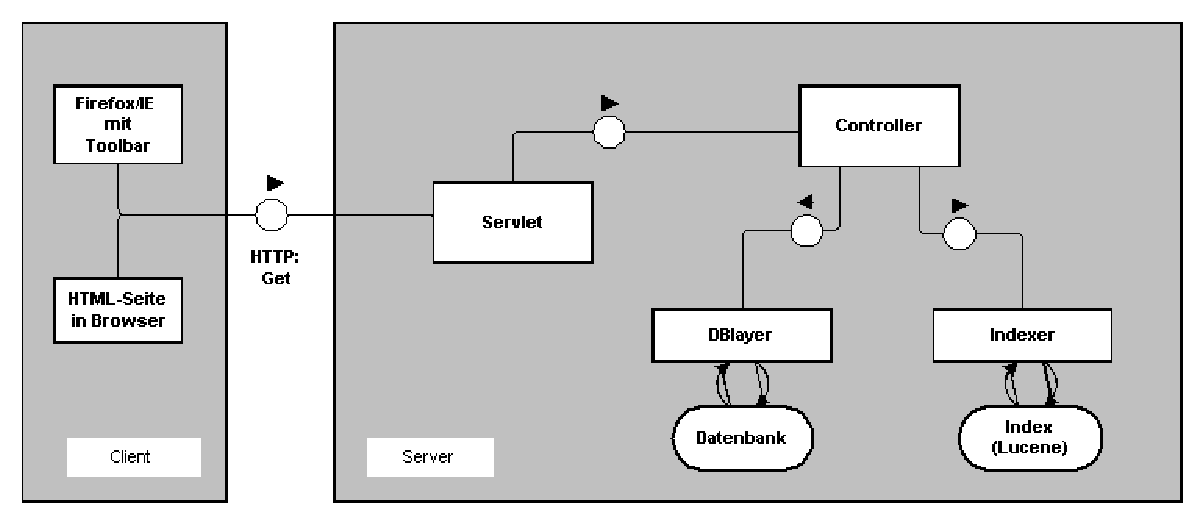
\includegraphics[width=16cm]{bilder/aufbau2.eps}
\caption{grobe ServerArchitektur}
\label{serverarchgrob}
\end{figure}




\subsection{Servlet}
\label{servlet}
Das Servlet ist der Einstiegspunkt f�r jegliche Anfragen an TeamFound. Dem Servlet kommt dabei die Rolle eines W�chters zu, welcher �berpr�ft ob notwendige Parameter f�r die einzelnen Anfragen vorhanden sind. Ist eine Anfrage g�ltig, wird diese an den sogenannten Controller weitergereicht, welcher die eigentlichen TeamFound-Komponenten steuert. Dieser Controller gibt immer ein Response-Objekt zur�ck, welches vom Servlet dann zB. als XML oder HTML serialisiert und als Antwort zum Client geschickt wird.

\subsection{Controller}
\label{controller}
Die Hauptaufgabe des Controllers besteht darin die Teilaufgaben, die sich aus einer 
Anfrage ergeben, koordiniert an Datenbank und Index zu stellen.
Ausserdem sorgt er f"ur den Download der zu indizierenden Dokumente.

Die Zugriffe auf den Index werden dabei durch eine Instanz eines Indexers erledigt.
Um die Zugriffe der Indexer auf den Index zu steuern, besitzt der Controller ein
Semaphorobjekt. Dieses realisiert eine Leser-Schreiber-Kooperation der beauftragten
Indexer.

Der Zugriff auf die Datenbank erfolgt "uber den DBLayer. Dieser stellt
s"amtliche Funktionalit"at zum lesen und schreiben der Datenbank zur
Verf"ugung.

Wenn alle Teilaufgaben erf"ullt sind (siehe Abl"aufe \ref{request}), generiert der Controller aus den 
erhaltenen Informationen eine Response und "ubergibt diese dem Servlet.

\subsection{Indexer}
\label{indexer}
Der Indexer ist f"ur die Arbeit direkt am Lucene-Index verantwortlich. Er f"ugt 
Dokumente (siehe \ref{lucene}) in den Index ein oder entfernt sie wieder. 
Ausserdem f"uhrt er Suchanfragen auf dem Index aus.
Die von uns definierte Dokumentenstruktur (siehe \ref{docstruktur}) ist bereits im Cotroller bekannt, 
somit kann der Indexer vorgefertigte Dokument erhalten und als Ergebnis liefern. 
Zur Indizierung und zur Suche benutzt der Indexer 
einen eigenen Analyzer (siehe \ref{lucene}), 
der wird haupts"achlich ben"otigt um das Kategorienfeld (siehe \ref{docstruktur}) korrekt zu zerlegen.
Ausserdem geh"ort ein einfacher Html-Parser zum Indexer, dieser soll den Text und
einige zus"atzliche Informationen (z.b. context-type) aus den Html-Seiten extrahieren.
Weitere Parser z.b. f"ur Postscript oder Pdf-Files sind in zuk"unftigen Versionen denkbar.

Die Anfragen werden zu eiem teil durch den QueryParser (siehe \ref{lucene}) und zum 
anderen vom Indexer generiert. Der Indexer erstellt dabei die Einschr"ankung
welche Kategorien in der Anfrage g"ultig sind.
Aus beiden teilen wird die gesammte Anfrage gebildet und an den Index gestellt.
Die Verarbeitung der Ergebnisse "ubernimmt der Controller.

\subsection{Response}
\label{response}
Antworten werden in TeamFound immer als XML generiert, diese XML\-Repr�sentation kann bevor sie zum Client geschickt wird, noch mittels XSLT in eine geeignete HTML\-Fassung gewandelt werden.
Eine Basisklasse Response �bernimmt dabei das Handling des eigentlichen JDOM-Document-Objektes, w�hrend die eigentlichen Antwort\-Klassen, wie SearchResponse oder AddPageResponse ihre eigentlichen Inhalte an die Standardelemente einer Antwort anh�ngen (Siehe dazu mehr im Kapitel Protokoll TODO: LINK).


\section{Datenmodell}
In diesem Kapitel soll auf die Datenstrukturen in der
Datenbank und im Index eingegangen werde.

Ausserdem soll erl"autert werden, warum Daten auf diese Weise zwischen Index und 
Datenbank verteilt wurden und wo Zusammenh"ange bestehen.
Dabei wird das Hauptaugenmerk auf die Struktur der Kategorienrepr"asentation gelegt.
In sp"ateren Versionen von Teamfound wird an dieser Stelle sicherlich auch das Problem
von Nutzer- und Rechtemanagement zu kl"aren sein.

\subsection{Datenbank}
\label{datenbank}

\begin{figure}
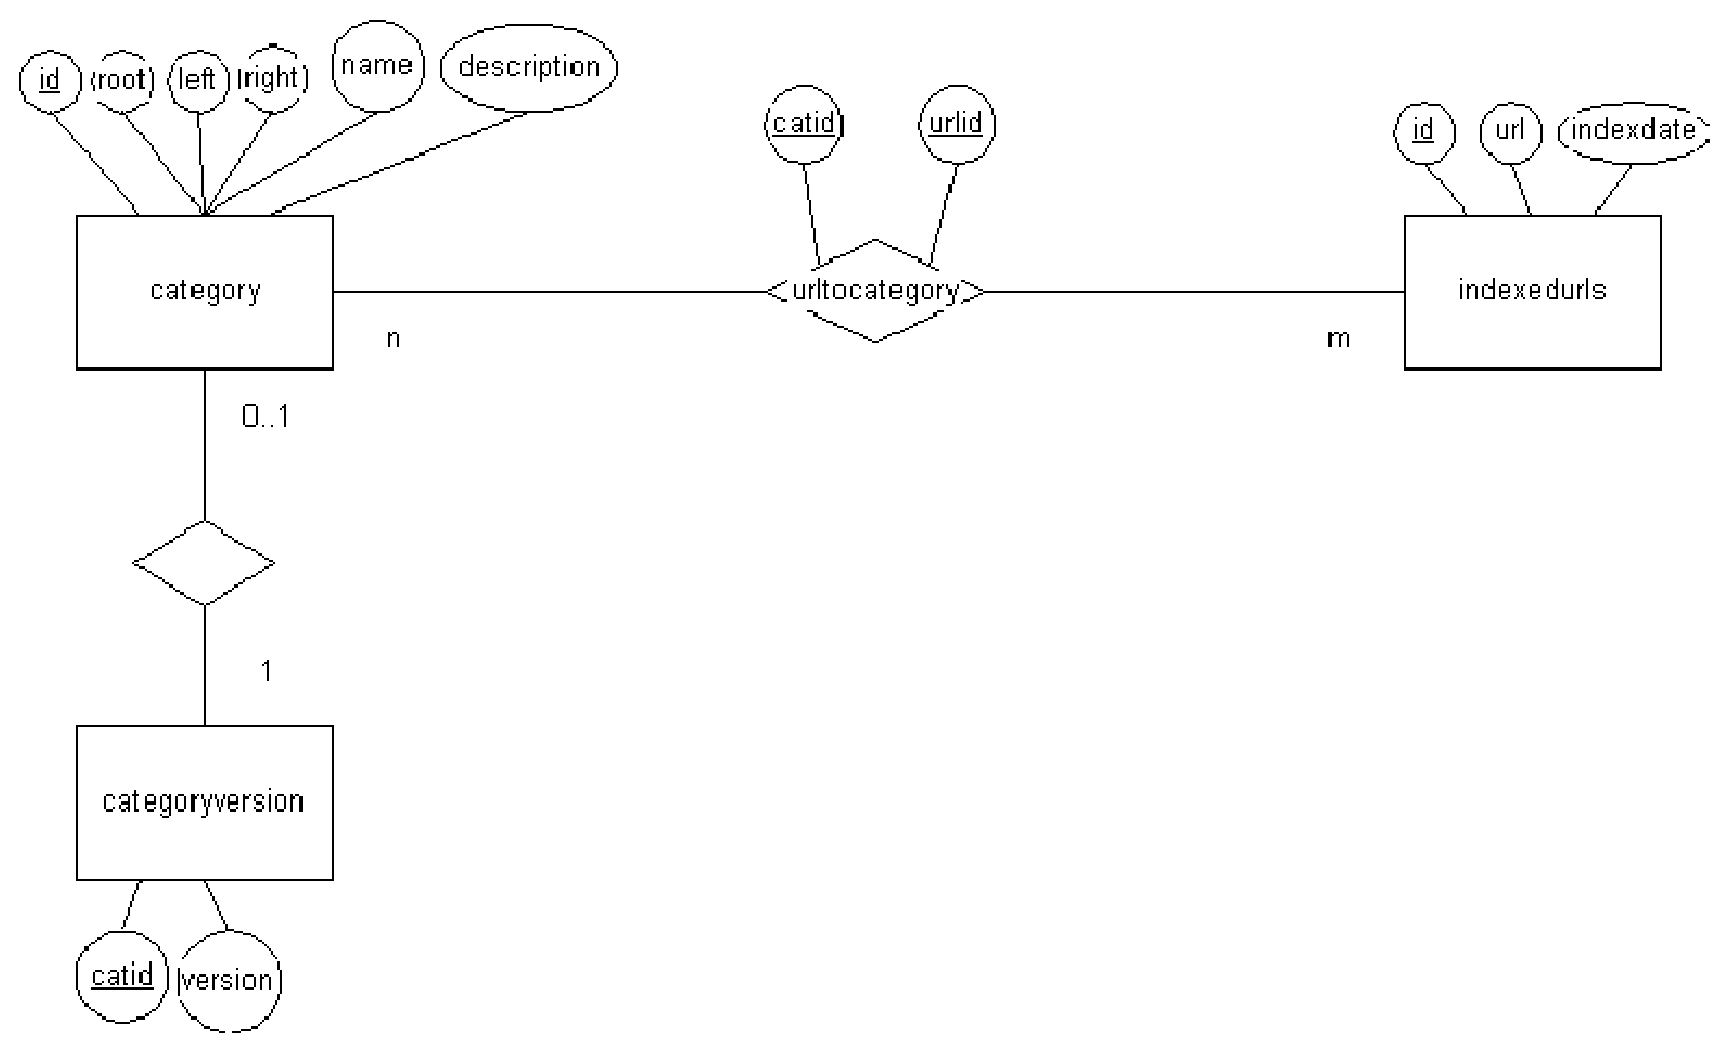
\includegraphics[width=16cm]{bilder/db.eps}
\caption{Datenbank-ERD}
\label{dberd}
\end{figure}

Die Datenbank besteht zur Zeit aus 4 Tabellen (siehe Abbildung \ref{dberd}).
Die wichtigste Tabelle des derzeitigen Standes ist die $category$-Tabelle.
Sie beinhaltet die Kategorieb"aume der Projekte eines Servers.

Um die B"aume in der Datenbank zu repr"asentieren haben wir
Verschachtelte Mengen (nested sets) eingesetzt. 
Dadurch k"onnen wir mit einfachen \texttt{select}-statements den
Baum durchsuchen, allerdings ist das einf"ugen oder edititeren des Baumes aufwendig.
Da wir Serverseitig haupts"achlich Suchvorg"ange zu bedienen haben, wollten wir
eine Rekursive Tabellenstruktur in der Datenbank vermeiden.
Die Verschachtelten Mengen boten uns eine gute Variante dies zu umgehen.
Genauere Informationen hierzu befinden sich im Kapitel \ref{katrep} .

Die Tabelle $categoryversion$ k"onnte prinzipiell zu jeder Kategorie eine
Versionsnummer mitf"uhren. Derzeit wird dies nur f"ur Wurzelknoten getan.
Damit hat jeder vom Server verwaltete Kategoriebaum eine Versionsnummer. Diese
wird benutzt um die Aktualit"at der B"aume zwischen Clienten untereinander 
und mit dem Server sicherzustellen.
Es ist durchaus vorstellbar Versionsnummern bei gro"sen Projekten
auch f"ur Teilb"aume zu verteilen, was derzeit aber nicht geplant ist.

Zu jeder Kategorie k"onnen beliebig viele Urls zugeordnet werden. Diese
werden in der $indexedurl$ Tabelle gehalten. Jede Url, die indiziert wurde, wird
mit Datum in dieser Tabelle gespeichert. Somit kann schnell festgestellt werden,
ob eine Url schon einmal hinzugef"ugt wurde und zu welchen Kategorien sie bisher
zugeordnet war.
Da der Index selbst auch doppelte Eintr"age zul"asst, 
ist es wichtig vor dem Einf"ugen das vorhandensein "uberpr"ufen zu k"onnen. 

Jede Url kann auch beliebig zu Kategorien zugeordnet werden,
da wir dieselbe Url in verschiedenen Kategorieb"aumen oder 
auch in verschiedenen Kategorien in ein und demselben Baum zulassen m"ochten.
Die Nutzer von Teamfound entscheiden in welche Kategorie ein Document 
geh"ort. Unabh"angig davon w"are eine "Uberpr"ufung, ob solch eine Zuordnung sinnvoll 
ist, auch kaum umzusetzbar.

Im Index wird allerdings zu jeder Url nur ein einziges Dokument (siehe \ref{luckomponenten}) abgelegt.
Wichtig ist dabei, dass eine Url, die einer Kategorie hinzugef"ugt wird, 
auch allen zugeh"origen Elternkategorien zugeordnet wird.
Das passiert in der Datenbank als auch im Dokument des Indexes.
Dadurch werden bei einer Suchanfrage innerhalb einer Kategorie automatisch 
auch alle Urls geliefert, die Kindkategorien dieser Kategorie zugeordnet wurden.

Das Datum in der $indexedurl$ Tabelle wird genutzt um Urls zu erkennen, welche
schon lange im Index liegen. Diese werden dementsprechend neu indiziert.



\subsection{Index und Dokumentstruktur}
\label{docstruktur}

Die Bibliothek Lucene macht bestimmte Vorgaben wie die Textdokumente, die von Lucene
indiziert werden sollen, zu erstellen sind. (siehe \ref{luckomponenten})

In diesem Abschnitt soll kurz der Aufbau eines von Teamfound erstelltem Dokuments
beschrieben werden. Zur Hilfestellung lohnt es sich Abbildung \ref{katstruktur} 
anzuschauen.

Jede Html-Seite, die dem Index hinzugef"ugt werden soll, muss erstmal serverseitig heruntergeladen werden.
Danach wird der Text und weitere Informationen extrahiert.
Dies alles, sowie die Kategorien zu denen die Seite zugeordnet wurde, wird nun in 
ein Lucene-Dokument verpackt.

Das erste Feld (siehe \ref{luckomponenten}), welches ein Teamfounddokument 
enth"alt, ist
ein Schl"usselwortfeld. In diesem wird die Url zu der dieses Dokument geh"ort
gespeichert. Dieses Feld wird nicht durch den Teamfound-$Analyser$ (siehe \ref{luckomponenten}) zerlegt, aber durchsuchbar im Index abgespeichert. 
Die Url wird also zur eindeutigen Identifikation eines Dokumentes ben"otigt. 
Zus"atzlich ist es m"oglich den Index nach Urls zu durchsuchen.

Als n"achstes speichern wir eine sehr kurze Zusammenfassung. 
Diese wird weder zerlegt noch indiziert. 
Sie dient ausschlie"slich als n"ahere Beschreibung eines Suchergebnisses einer Anfrage.

Ein weiteres Feld ist der Titel der Seite. Er wird zerlegt und indiziert.
Anfragen die Schl"usselw"orter enthalten, die im Titel vorkommen, erhalten
dadurch eine h"ohere Wertigkeit.

Das wichtigste Feld neben der Url enth"alt den textuellen Inhalt der Seite.
Dieser wird in Token zerlegt und indiziert.
Anfragen an den Index durchsuchen grunds"atzlich dieses Feld und das Titelfeld.

Die Ergebnisse solcher Anfragen sollen nun durch Kategoriezugeh"origkeit
eingeschr"ankt werden. Daf"ur umfassen Teamfounddokumente ein weiteres Feld, dass
die Kategorien enth"alt denen das Dokument zugeordnet wurde. 

Die Anfrage "uber Inhalt und Titel wird also
mit einer zweiten Suchanfrage "uber dem Kategorienfeld verkn"upft und eingeschr"ankt.
Um solche Anfragen zu erm"oglichen muss jedes Token in einem Kategoriefeld eindeutig
einer Kategorie zuzuordnen sein.

Die einfachste L"osung war die ID einer Kategorie aus der Datenbank als Token 
zu benutzen, und diese in dem Kategoriefeld zu speichern.
Damit es m"oglich ist die verschiedenen IDs zu unterscheiden, trennen wir diese mit 
einem eindeutigen Charakter voneinander ab.
Den Teamfound-$Analyser$ haben wir dementsprechend angepasst,
so dass er die Tokens dieses Feldes einfach anhand des Trenncharakters generiert.
Auf diese Weise k"onnen wir die Anfragen leicht so erweitern, dass sie mithilfe von Kategorien eingeschr"ankt werden k"onnen.


\subsection{Repr"asentation der Kategorien}
\label{katrep}

\begin{figure}
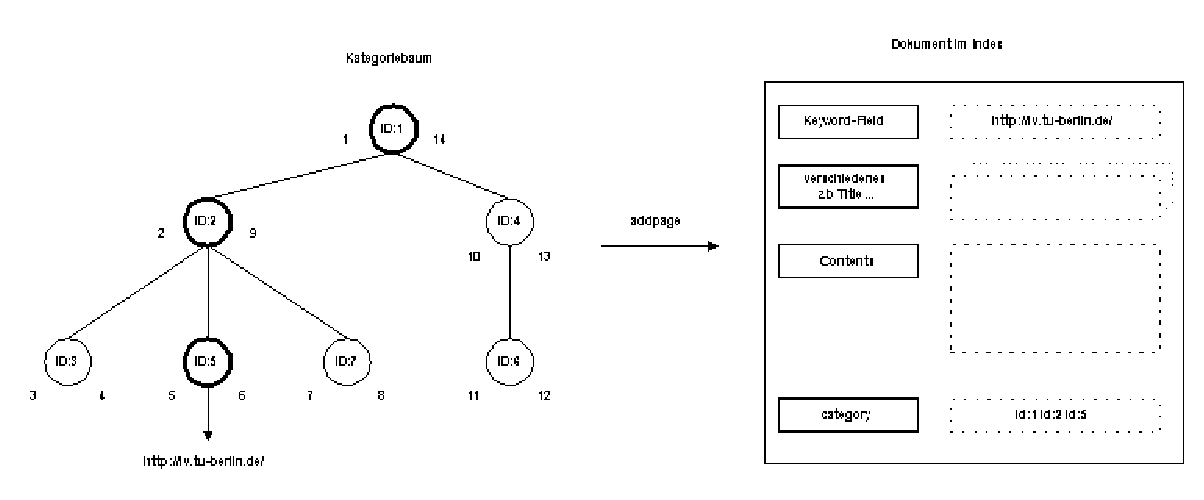
\includegraphics[width=16cm]{bilder/katstruktur.eps}
\caption{Repr"asentation der Kategorien in DB und Index}
\label{katstruktur}
\end{figure}

Da ein wichtiger Teil des derzeitigen Servers die Verwaltung der Kategorien 
betrifft, soll hier noch einmal etwas genauer auf diese eingegangen werden.

Wie schon in Kapitel \ref{datenbank} erw"ahnt wurde sind die Kategorien 
baumstrukturiert und werden in Form von Verschachtelten Mengen in der
Datenbank abgelegt.
Die grafische darstellung eines solchen Baumes und einer solchen Menge
kann man in Abbildung \ref{katstruktur} sehen. 
Es ist leicht zu erkennen, dass alle Knoten des Baumes einen linken und
einen rechten Wert aufweisen. 
Anhand dieser Werte kann die Mengen- Baumstruktur in der Datenbank nachgebaut und 
der Baum durchlaufen werden.
Es ist leicht zu erkennen, dass der rechte Wert eines Knotens gr"o"ser ist als
alle Werte der Kindknoten und genauso ist der linke Wert kleiner.
Es gelten noch einige andere n"utzliche Dinge, z.b.  
k"onnen alle Bl"atter des Baumes sehr leicht indentifiziert werden, da
bei diesen die Differenz von linkem und rechtem Wert einfach 1 betr"agt.

Wir haben diese Struktur ausgew"ahlt, weil das durchsuchen 
sehr einfach und schnell geht. 
Der grosse Nachteil ist das Ver"andern eines solchen Baumes. Damit die Struktur
in Takt bleibt muss prinzipiell jeder Knoten der ''rechts'' des bearbeiteten Knotens
liegt angepasst werden. Dies wird bei sehr tiefen B"aumen entsprechend aufwendig.

Das sollte f"ur unseren Anwendungsfall aber kein Problem sein. Die Kategorien  
werden von Nutzern der "Ubersichtlichkeit halber angelegt und sollten deshalb 
wohl nicht so tief und stark verzweigen.
Ausserdem gehen wir davon aus, dass das ver"andern der Kategorien 
eher selten vorkommen wird. Wenn ein neues Projekt beginnt werden in der Anfangsphase 
von den Mitgliedern sicher einige Kategorien angelegt, diese 
werden danach aber auch nahezu unver"andert bleiben.

Auf der anderen Seite muss bei sehr vielen Anfragen der Baum durchsucht werden.
Allein das Anlegen einer neuen Kategorie hat zur Folge, das jeder Client den
neuen Kategorienbaum vom Server erfragt.
Da wir also den Baum sehr oft auslesen m"ussen ist diese Art der Speicherung vorteilhaft.
Hinzu kommt, das es sehr aufwendig ist einen solchen Baum oder Pfade 
eines Baumes in einem Index abzulegen.
Deshalb speichern wir im Index auch nur eine einfache Aufz"ahlung 
von Kategorien ab. (siehe Abbildung \ref{katstruktur} und Kapitel \ref{docstruktur})
Diese enth"alt zwar den ganzen Pfad, dennoch l"asst sich dieser nicht
wiederherstellen, da ja mehrere Pfade in der Aufz"ahlung enthalten sein k"onnen.
Es entsteht dadurch aber kein Problem. Eine Suchanfrage an den Server ben"otigt trozdem keinen
Datenbankzugriff, sondern kann mit einer Anfrage an den Index bearbeitet werden.
(siehe Kapitel \ref{searchrequest}) 
Das l"asst sich mit dem Zweck unserer Anwendung erkl"aren. 
Wir stellen eine Suche anhand von Suchbegriffen bereit. Die Kategorien sind nur
eine Einschr"ankung der Suchergebnisse. 
Je allgemeiner die Kategorie in einer SuchAnfrage gew"ahlt wird,
desto mehr Ergebnisse werden gefunden.
Das erkl"art sich darin, das alle Dokumente, die einer Unterkategorie 
angeh"oren, auch allen Elternkategorien zugeordnet wurden.
Dieser einfache Trick erreicht genau unseren Zweck.
Bei einer Suchanfrage wird ein Dokument in jeder Kategorie, die auf dem Pfad 
durch den Baum liegt gefunden und sie kann schnell ausgef"uhrt werden.


\section{Abl"aufe im Server}
\label{request}
Wie Aufrufe vom Client im Server abgearbeitet werden, soll kurz in diesem Abschnitt 
behandelt werden.
Wir haben drei verschiedene Serverdienste ausgew"ahlt. Sie sollen einen Einblick in die
Interna des Servers bieten und dadurch die Funktionsweise von Teamfound noch
etwas besser verst"andlich machen.


\subsection{AddpageRequest}
\label{addpagerequest}

\begin{figure}
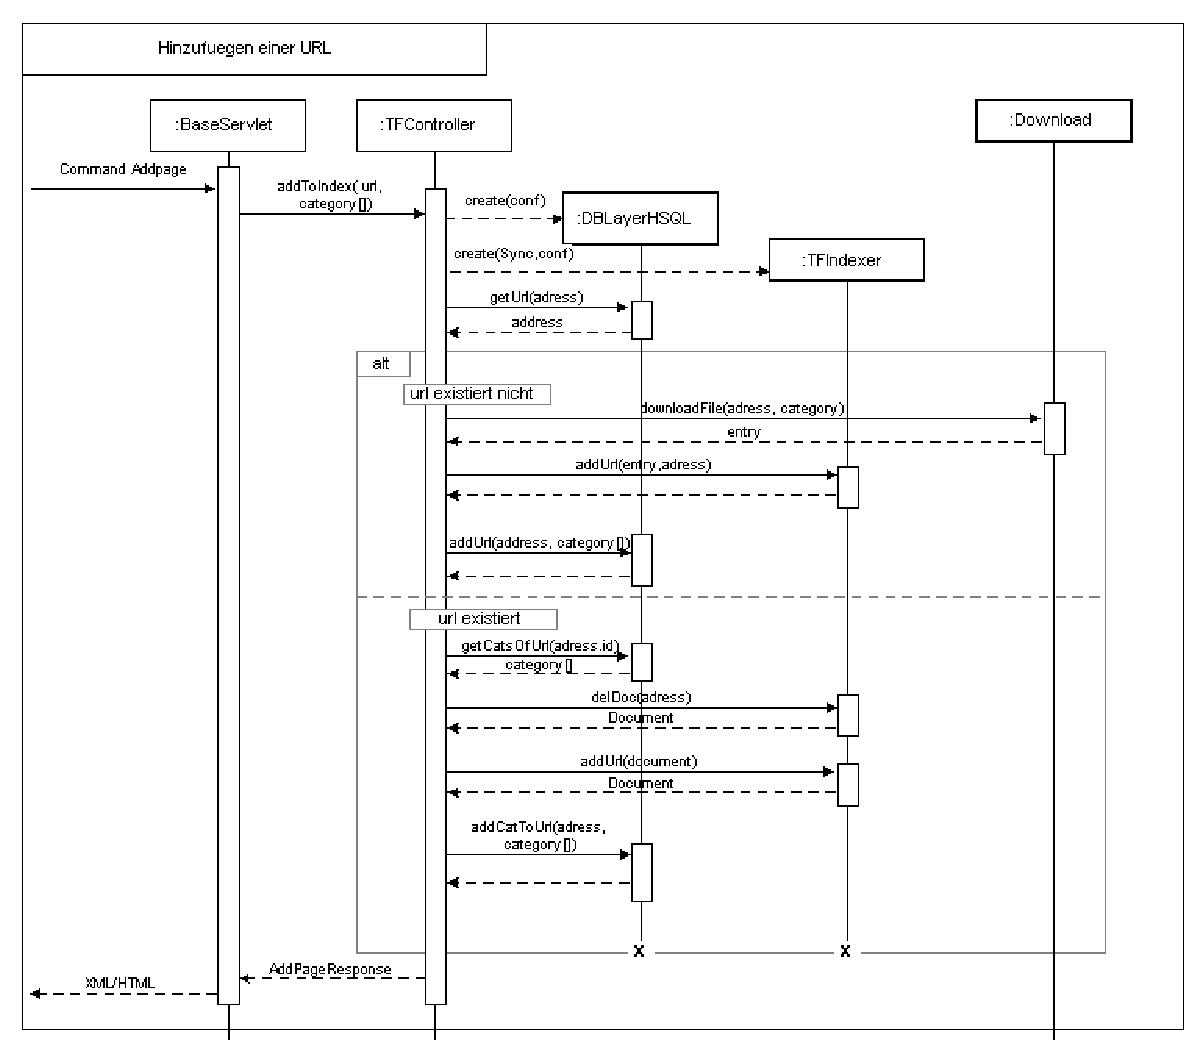
\includegraphics[width=16cm]{bilder/ablaufaddpage1.eps}
\caption{Indizieren einer neuen URL}
\label{addpage}
\end{figure}

Die wichtigsten Funktionen von Teamfound sind ohne Zweifel, dass hinzuf"ugen und
das Suchen. Deshalb soll als erstes ein Einblick in das Hinzuf"ugen von Urls 
gegeben werden. Hierzu liefert die Abbildung \ref{addpage} einen "Uberblick.

Der Aufruf des Clients wird in $Get$-Variablen in der Url codiert (siehe \ref{interface2})
und vom Servlet (siehe \ref{servlet}) entgegengenommen. 
Ist der Aufruf korekt, d.h. er enth"alt die hinzuzuf"ugende Url und mindestens 
eine Kategorie, wird der Controller (siehe \ref{controller}) mit entsprechendem 
Auftrag angestossen.
Bei nicht korekten Aufrufen wird eine \texttt{ErrorResponse} erstellt.

Der Controller erstellt nun eine Verbindung zur Datenbank 
und einen Indexer (siehe \ref{indexer}).
Als n"achstes "uberpr"uft er anhand der Datenbank ob die Url schon existiert.
An dieser Stelle ergeben sich zwei M"oglichkeiten.
Sollte die Url noch nicht indiziert sein, so muss sie als erstes runtergeladen werden.
Danach wird ein Dokument erstellt und durch den Indexer dem Index hinzugef"ugt.
(siehe hierzu Kapitel \ref{docstruktur})
Als letztes muss noch die Datenbank angeglichen werden. (siehe Kapitel \ref{datenbank})

Die zweite M"oglichkeit ist, dass die Url bereits indiziert wurde.
Um ein Update der Url im Index durchzuf"uhren, muss zuerst das entsprechende Dokument
aus dem Index gel"oscht werden. Dabei wird eine Kopie des Dokuments an den Controller
geliefert. Dieser ersetzt nun das Kategorienfeld (siehe Kapitel \ref{docstruktur}), damit
die neuen Kategorien auch enthalten sind.
Danach wird das Dokument dem Index wieder hinzugef"ugt und die entsprechenden neuen
Assoziationen zwischen Url und Kategorien werden in der Datenbank gesetzt.

Es gibt noch eine dritte M"oglichkeit, die allerdings in Abbildung \ref{addpage} nicht
dargestellt ist. Die Url ist bereits hinzugef"ugt und es ver"andert sich auch bei
den Kategorien nichts. Auch diese M"oglichkeit wird anahnd der Datenbank "uberpr"uft.
Sollte der Fall eintreten passiert gar nichts und die Erfolgsmeldung wird 
sofort an den Client gesendet. Es ist einfach vorstellbar, dass ein Benutzer ausversehen
mehrmals das Hinzuf"ugen ausl"ost. In solch einem Fall wollen wir nicht unn"otig den
Index blockieren.
Allerdings gibt es auch hier eine Aussnahme. Sollte die Url ein gewisses ''Alter'' 
"uberschreiten wird sie auf jeden Fall erneut heruntergeladen.


\subsection{Ablauf SearchRequest}
\label{searchrequest}

\begin{figure}
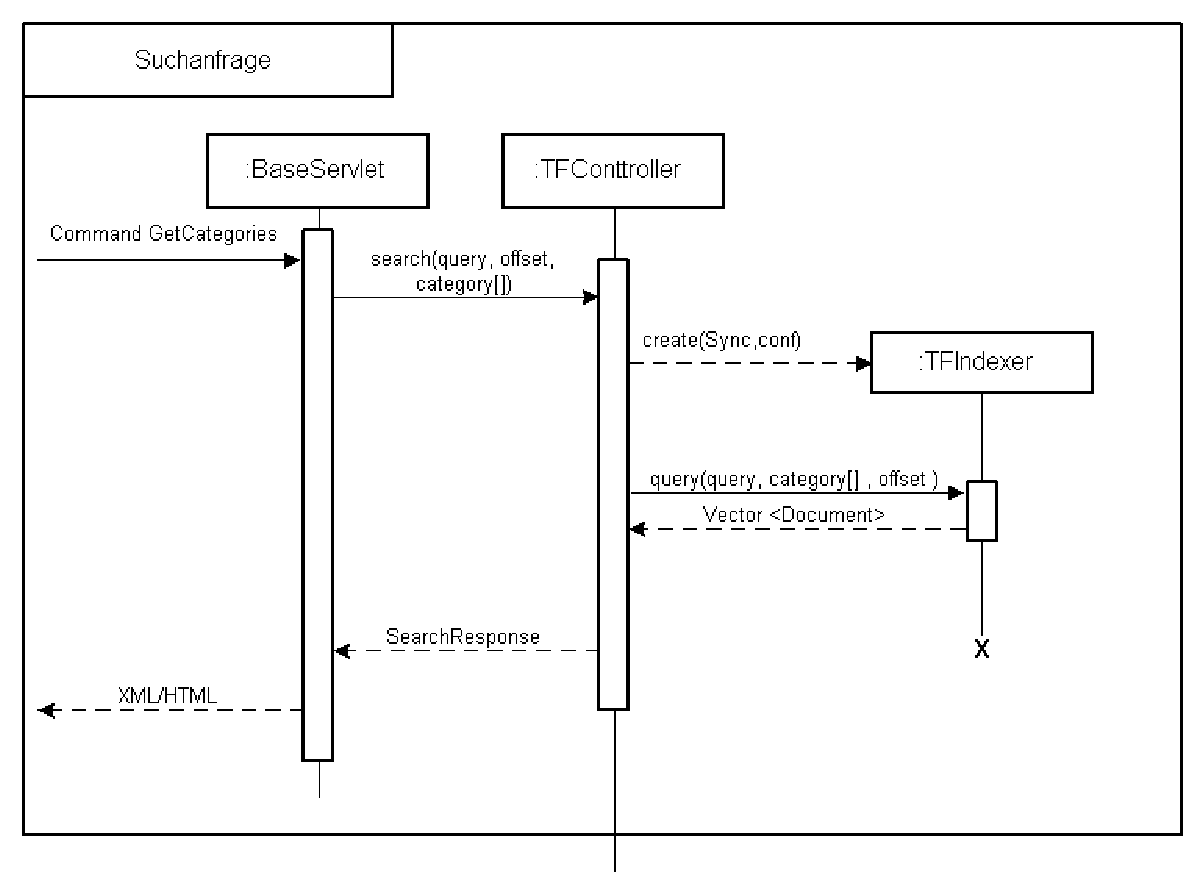
\includegraphics[width=14cm]{bilder/search.eps}
\caption{Suchanfrage an den Server}
\label{search}
\end{figure}



\subsection{Ablauf GetCategoriesRequest}
\label{getcatrequest}

\begin{figure}
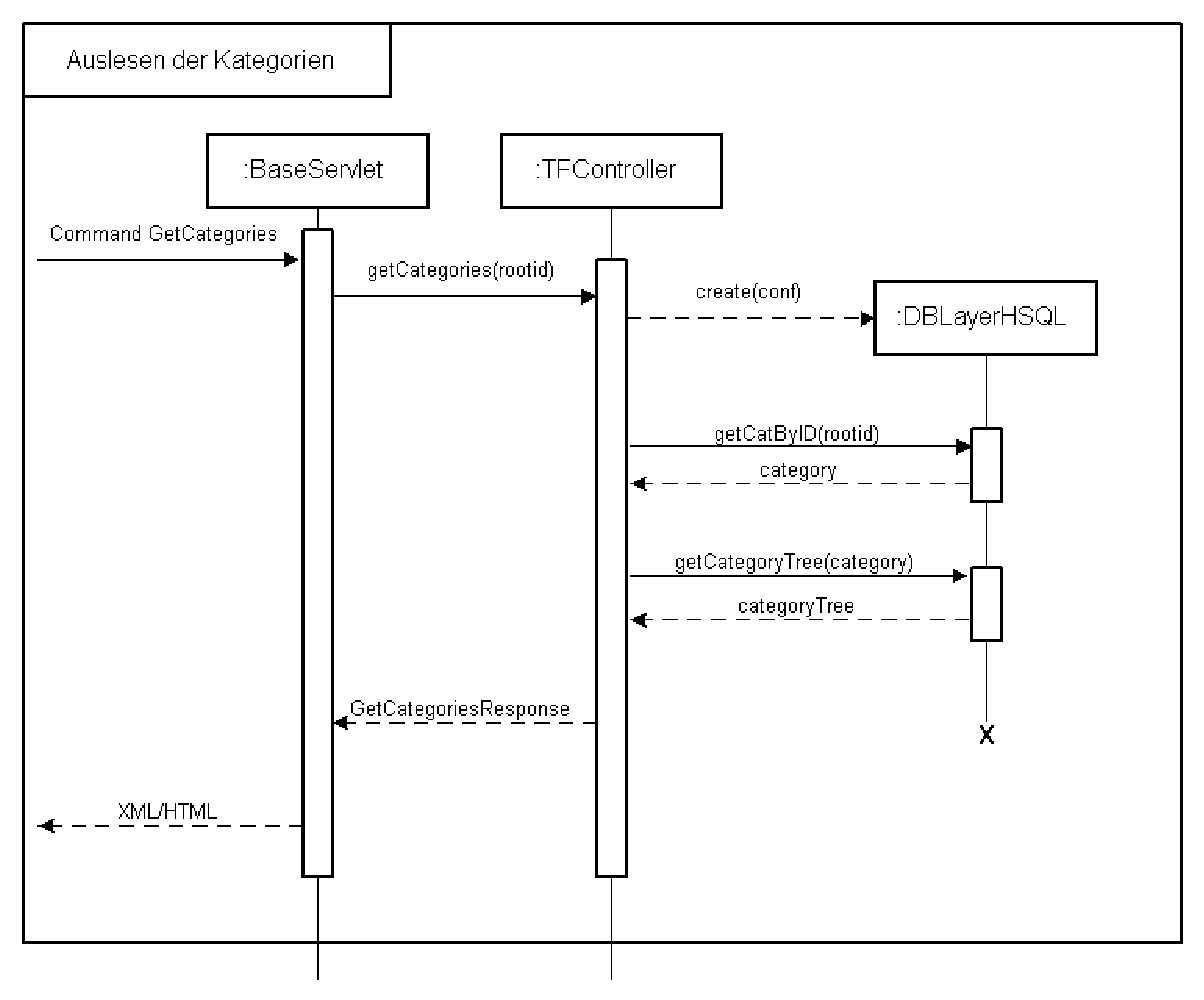
\includegraphics[width=14cm]{bilder/getcat.eps}
\caption{Abfragen der Kategorien}
\label{getcat}
\end{figure}



\chapter{Protokoll}
Die in unserem Projekt von Anfang wohl grundlegendste Frage war die des Protokolls, also wie unsere Clients mit dem Server kommunizieren sollen. Auf jeden Fall sollte ein Protokoll spezifiziert werden, welches um sp"atere, jetzt noch unbekannte Features, m"oglichst leicht erweiterbar sein sollte. Es sollte ausserdem gut Dokumentiert und eindeutig sein, damit "ahnliche Projekte, die die Idee hinter TeamFound ebenfalls implementieren wollen, \textbf{motiviert werden} dasselbe Protokoll zu benutzen. Somit k"onnten dann Server und Clients aus unterschiedlichen Projekten miteinander funktionieren und arbeiten.

Wir sind uns nicht sicher, wie weit wir diese Ziele mit Milestone 2 bereits erreicht haben, aber wir glauben auf dem richtigen Weg zu sein ;-)

\section{Designentscheidungen und verwendete Techniken}
F"ur unser Protokoll kamen prinzipiell viele verschiedene M"oglichkeiten in Betracht. 

Die erste, und einfachste Designentscheidung war, ein Protokoll zu benutzen, welches auf TCP/IP aufsetzt. Somit k"onnen schonmal alle Computer die "uber einen Internet-Zugang verf"ugen prinzipiell mit unseren Componenten kommunizieren.

Der zweite Schritt war die Festlegung unseres Protokolls nicht direkt auf TCP/IP aufzusetzen, sondern erst auf dem HTTP Protokoll. Diese Entscheidung viel auch sehr schnell und war f"ur uns naheliegend, da wir von Anfang an vorhatten Browser-Plugins zu programmieren, und jeder Internet-Browser HTTP ebenfalls unterst"utzt. 

Als weitere Grundlage f"ur unsere Designentscheidungen war unser Wunsch, die M"oglichkeit einen ganz einfachen Web-Client bereitstellen zu k"onnen, so da"s TeamFound auch ohne Installation einer Browser-Erweiterung ausprobiert und genutzt werden kann. Diese Entscheidung f"uhrte dann auch direkt zu der eigentlichen Basis unseres Protokolls:
\begin{description}
\item[HTML-Antworten des Servers] Somit kann jeder Browser die Suchergebnisse unseres Servers direkt anzeigen.
\item[Anfragen an Server mittels HTTP-GET Variablen] Somit kann ein einfaches HTML-Formular korrekte Suchanfragen an unseren Server stellen.
\item[XML-Antworten des Servers] Diese M"oglichkeit, konfigurierbar "uber die Suchanfrage, erm"lglicht den Browser-Plugins, und somit dem End-Benutzer, die Darstellung der Suchergebnisse selber zu beeinflussen bzw. komplett anzupassen.
\end{description}

Die Implementierung des Protokolls, sowie auch alle anderen Komponenten von TeamFound, hatte wir in kleine Schritte unterteilt, unsere Milestones. So hat das Protokoll f"ur Milestone 1 z.B. noch keine Unterst"utzung f"ur XML-Antworten und Kategorien gehabt.

Auf Basis dieser gundlegenden Entscheidungen, haben wir also begonnen sowohl die HTTP-GET Anfragen zu spezifizieren als auch (ab Milestone 2) XML-Tags zu definieren, um die volle Funktionalit"at unserer Implementation nutzen zu k"onnen. 

\section{Interface Milestone 1}

\subsection{Seite hinzuf�gen}
\begin{description}
\item[Request] http://url/addpage.pl?url=http://yy.org/blabla.html
\item[Antwort] keine
\end{description}

\subsection{Suchen}
\begin{description}
\item[Request] http://url/search.pl?keyword=zzz
\item[Antwort] HTML-Seite mit URLs gefundener "Ubereinstimmungen 
\end{description}

\section{Interface Milestone 2}
\label{interface2}
\subsection{Allgemein}
\subsubsection{Tests}
Zum Testen der Serverseitigen Interface-Implementation existiert folgende Webseite, die entsprechende Requests erstellen kann: 

\texttt{http://teamfound.berlios.de/test\_the\_server\_interface\_m2.html}
\\
\\
Zum Testen der Clientseitigen Interface-Implementation existiert folgendes Perl-Skript, welches den Parameter command auswertet und eine enstsprechende statische XML-Antwort zurueckgibt: 
\\
\texttt{http://teamfound.dyndns.org/interface-m2/testmilestone2.pl}
\\
Demo: 
\\
\texttt{http://teamfound.dyndns.org/interface-m2/testmilestone2.pl?command=getcategories}
\\
Das Skript liegt auch im SVN unter \texttt{teamfound/interface/milestone2/testmilestone2.pl}

\subsubsection{Alle Anfragen an den Server}

Alle Anfrage-Parameter werden in Form von HTTP GET oder POST Variablen �bertragen. Prinzipiell gibt es eine Unterscheidung, ob f"ur jedes Kommando eine eigene URL verwendet wird, oder ob das Kommando in Form einer weiteren HTTP-GET Variablen mit "ubertragen wird. Unsere Implementation des  Servers verwendet den zus"atzlichen HTTP-GET Parameter \texttt{command}. In diesem Interface haben wir aber beide M"oglichkeiten spezifiziert.

\begin{description}
\item[want=xml or html] Die zu erwartende Antwort soll in xml oder html-format sein (default soll html werden, da dann einfache Link-Clients m�glich sind) 

\item[version=2] Milestone-Version des Interfaces 

\item[command=search] Das Kommando das ausgef�hrt werden soll. Dieses Argument kann wegfallen wenn f�r jedes Kommando eine eigene, gleichnamige Anfrage-URL existiert. 
\end{description}

\subsubsection{HTML-Antwort}
Die Clients geben an ob Sie eine HTML oder eine XML Antwort erwarten.

Soll eine vollst�ndige HTML-Seite zur�ckgeben, die direkt im Browser angezeigt werden kann. Die Return-Values wie bei einer XML-Antwort m�ssen in diesem Fall nicht zur�ckgegeben werden, sondern der Text sollte gleich eine entsprechende Meldung beinhalten.

\subsubsection{XML-Antwort}
\begin{description}
\item[$<$response$>$] Umschliesst alle anderen xml-tags und gibt die XSD-Datei zum verifizieren der XML-Daten an 
\item[$<$interface-version$>$] Gibt immer die Interface-Version an, in der die Antwort des Servers formuliert wurde 
\item[$<$server$>$] Gibt Name und Versionsnummer des Servers an. Der Server der unter der URL https://developer.berlios.de/projects/teamfound entwickelt wird gibt den Namen "TeamFound" zur�ck. Clones d�rfen Ihren eigenen Namen nat�rlich frei w�hlen. 
\item[$<$addpage$>$ $<$search$>$ $<$addcategory$>$ $<$getcategories$>$] Diese Tags beinhalten die Antworten auf die gleichnamigen Anfragen an den Server. Pro Anfrage darf nur eines dieser Tags vorkommen. 
\item[$<$return-value$>$ $<$return-description$>$] Der Return-Value bzw. Fehler-Code falls etwas schiefging. Die Description wird nicht genauer spezifiziert, sollte aber semantisch mit dem aufgetretenen Fehler �bereinstimmen. 
\item[$<$project-counter$>$] Bei jeder �nderung des Kategorien-Baumes(Graph!) soll der Server einen internen Z�hler um eins inkrementieren. Der aktuelle Wert soll bei jeder XML-Antwort mit �bertragen werden. (Dann weiss die Toolbar wann sie selber die Kategorien neu vom Server abfragen muss.)Jedes Projekt fuehrt einen Counter, somit muss der Client nur die fuer ihn intressanten Baeume beachten. 
\end{description}

\begin{verbatim}
<response xmlns:xsi="http://www.w3.org/2001/XMLSchema-instance"
xsi:noNamespaceSchemaLocation="teamfound-interface-milestone2.xsd">

 <interface-version>2</interface-version>

 <return-value>0</return-value>
 <return-description>OK</return-description>

 <project-counter>
   <project>
     <projectID>0</projectID>
     <count>3</count>
   </project>
   <project>
     <projectID>3</projectID>
     <count>5</count>
   </project>
 </project-counter>

 <category-counter>54</category-counter>

 <server>
  <name>TeamFound</name>
  <version>0.2</version>
 </server>

 <addpage>
 </addpage>

 <search>
 </search>

 <addcategory>
 </addcategory>

 <getcategories>
 </getcategories>
 
</response>
\end{verbatim}

\paragraph{Return Codes}

Die Return-Codes stehen immer in den Tags $<$return-value$>$xx$<$/return-value$>$. Die Description ist optional.

\begin{description}
\item[0] Alles ok 

\item[1] Fehler, konnte URL nicht finden 

\item[2] Ung�ltige Anfrage (Pflicht-Parameter fehlen oder haben die L�nge null) 

\item[3] Inkompatible Interface-Version (die Anfrage hat eine Interface-Version benutzt die der Server nicht unterst�tzt) 

\item[4] Kategorie existiert schon (beim hinzufuegen einer neuen Kategorie) 

\item[5] Kategorie nicht gefunden (beim suchen nach einer bestimmten Kategorie) 

\item[-1] Anderer Fehler 
\end{description}

Die Return-Descriptions sind frei w�hlbar, sollten aber dem Return-Code semantisch entsprechen ;-)


\subsection{Seite hinzuf�gen}
\subsubsection{Anfrage an Server}

\begin{description}
\item[command=addpage] Der Kommando-Name 

\item[addpage.pl] Der (default) Skriptname der die Anfrage entgegennimmt (dann f�llt das Argument command weg). 

\item[category=453] Die Kategorien-Nummer zu der der Link hinzugefuegt werden soll, in dieser Version nur genau eine oder keine. Wird keine Kategorie angegeben, so soll die Top-Kategorie genommen werden (also nicht gefunden werden wenn bei der Suche eine genauere Kategorie angegeben wird). 

\item[url=http://yy.org/blabla.html] Die zu indizierende url, das Protokoll ist mit anzugeben 
\end{description}

\subsubsection{XML Antwort}
xml oder html um �ber Erfolg oder Misserfolg zu berichten

Verwendet in der Antwort das XML-Tag: $<$addpage$>$
\begin{verbatim}
<response>

 <interface-version>2</interface-version>

 <return-value>0</return-value>
 <return-description>OK</return-description>

 <server>
  <name>TeamFound</name>
  <version>0.2</version>
 </server>

 <addpage>
  <url>http://blabla.html</url>
 </addpage>
 
</response>
\end{verbatim}

\subsubsection{HTML Antwort}
siehe Allgemeines zu HTML-Antworten


\subsection{Suchen}
\subsubsection{Anfrage an Server}
\begin{description}
\item[command=search] Der Kommando-Name 

\item[search.pl] Der (default) Skriptname der die Anfrage entgegennimmt (dann f�llt das Argument command weg). 
\item[keyword=zzz] Eine durch ' ' (space) getrennte Liste der Suchw�rter die alle vorkommen sollen (URL-Codiert mit ''\%20'' getrennt, also eine Suche nach auto und tv wird als keyword=auto\%20tv codiert). Dies beinhaltet eine serverseitig impliziete UND-Verkn�pfung aller Suchworte. Fehlt der Parameter so soll ein Fehler zur�ckgegeben werden. Die genaue Definition einer umfassenderen Suchanfragen-Sprache (wie OR, NOT etc.) ist noch festzulegen, wird aber auf spaetere Interface-Milestones verschoben. 

\item[category=5\&category=9\&category=15] Eine Liste aller Kategorien-IDs, jeweils immer wieder neu mit category= durch die die Suche gemacht werden soll. Fehlt der Paramater, so soll alles durchsucht werden. (Grund: HTML-Formulare machen dies bei Listen und ComboBoxen mit Mehrfachauswahl genau so). 
\end{description}

\subsubsection{XML Antwort}
Verwendet in der Antwort das XML-Tag: $<$search$>$

\begin{verbatim}
<response>

 <interface-version>2</interface-version>

 <return-value>0</return-value>
 <return-description>OK</return-description>

 <server>
  <name>TeamFound</name>
  <version>0.2</version>
 </server>

 <search>

  <keywords>
   <word>xxx</word>
   <word>yyy</word>
  </keywords>

  <result>

   <count>30</count>
   <offset>0</offset>

   <found>
    <url>http://xxx.html</url>
    <title>Der Titel der Seite</title>
    <incategory>5</incategory>
   </found>

   <found>
    <url>http://xxx.html</url>
    <title>Der Titel der Seite</title>
    <incategory>5</incategory>
   </found>

   <found>
    <url>http://xxx.html</url>
    <title>Der Titel der Seite</title>
    <incategory>5</incategory>
    <incategory>3</incategory>
    <incategory>7</incategory>
   </found>

  </result>
 </search>
 
</response>
\end{verbatim}
\begin{itemize}
\item Die Keywords sind zur Fehlerbehandlung alle nochmals mit anzugeben. 

\item Jeder gefundene Link wird in einem eingenen $<$found$>$ Block augegeben. 

\item Wurde kein Suchergebnis gefunden, so ist in $<$count$>$ die Anzahl 0 einzutragen, der Return-Code aber immernoch 0 (OK) wenn sonst alles ok war 
\end{itemize}

\subsubsection{HTML Antwort}
HTML-Seite mit URLs gefundener �bereinstimmungen

\subsection{Kategorien von Server abfragen}
\subsubsection{Anfrage an Server}

\begin{description}
\item[command=getcategories] Der Kommando-Name 
\item[getcategories.pl] Der (default) Skriptname der die Anfrage entgegennimmt (dann f�llt das Argument command weg). 
\item[projectID=5] Nummer des projekts f�r diese Anfrage 
\end{description}

\subsubsection{XML Antwort}
Verwendet in der Antwort das XML-Tag: $<$getcategories$>$
\begin{verbatim}
<response>

 <interface-version>2</interface-version>

 <return-value>0</return-value>
 <return-description>OK</return-description>

 <server>
  <name>TeamFound</name>
  <version>0.2</version>
 </server>

 <getcategories>
  <category>
   <name>name der kategorie</name>
   <description>laengere beschreibung</description>
   <id>0</id>
   <subcategories>
    <category>
     ...
    </category>
    <category>
     ...
    </category>
   </subcategories>
  </category>
 </getcategories>
 
</response>
\end{verbatim}

Hinweis: die Top-Kategorie hat immer die ID 0 (null) 

\subsubsection{HTML Antwort}
siehe Allgemeines zu HTML-Antworten

\subsection{Kategorie hinzuf�gen}
\subsubsection{Anfrage an Server}
\begin{description}
\item[command=addcategory] Der Kommando-Name 

\item[addcategory.pl] Der (default) Skriptname der die Anfrage entgegennimmt (dann f�llt das Argument command weg). 

\item[name=kategoriename] Den Namen den die neue Kategorie bekommen soll 

\item[subcategoryof=45] Die Kategorie der die neue Kategorie untergeordnet werden soll. Soll eine neue 1st-Level Kategorie erstellt werden ist hier 0 (null) anzugeben. 

\item[description] Eine etwas l�ngere Beschreibung der Kategorie (max. 255 Zeichen) 
\end{description}

\subsubsection{XML Antwort}
Verwendet in der Antwort das XML-Tag: $<$addcategory$>$
\begin{verbatim}
<response>

 <interface-version>2</interface-version>

 <return-value>0</return-value>
 <return-description>OK</return-description>

 <server>
  <name>TeamFound</name>
  <version>0.2</version>
 </server>

 <addcategory>
  <name>kategoriename</name>
  <gotid>53</gotid>
 </addcategory>
 
</response>
\end{verbatim}
\begin{itemize}
\item der neue Name
\item die ID die die neue Kategorie bekommen hat
\item name und gotid fallen weg wenn die kategorie schon existiert (return-value 4 - Kategorie existiert schon) oder die subcategoryof-id nicht existiert (return-value 5 - Kategorie nicht gefunden). 
\end{itemize}

\subsubsection{HTML Antwort}
siehe Allgemeine HTML-Antwort

\subsection{Alle Projekte auslesen}
\subsubsection{Anfrage an Server}
\begin{description}
\item[command=getprojects] Der Kommando-Name 
\item[addcategory.pl] Der (default) Skriptname der die Anfrage entgegennimmt (dann f�llt das Argument command weg). 
\end{description}

\subsubsection{XML Antwort}
Verwendet in der Antwort das XML-Tag: $<$projects$>$
\begin{verbatim}
<response>

 <interface-version>2</interface-version>

 <return-value>0</return-value>
 <return-description>OK</return-description>

 <server>
  <name>TeamFound</name>
  <version>0.2</version>
 </server>

 <projects>
   <project>
     <name>prjectname</name>
     <description>beschreibung</description>
     <id>7</id>
   </project>
   ...
 </project>
 
</response>
\end{verbatim}

\subsubsection{HTML Anwort}
siehe Allgemeine HTML-Antwort

\subsection{L�schen einer Kategorie}
Wird erst in Interface Milestone 3 implementiert werden. Es stellt sich die Frage was mit den in dieser Kategorie bereits befindlichen Links gemacht wird .. verschieben?


\chapter{Clients}

\section{Web-Client}
Der Web-Client ist ein einfaches HTML-Formular (\texttt{$<$form$>$..$<$/form$>$}), welches Anfragen an den Server sendet und die Antwort direkt im Browser anzeigt. Dieser Client ist von daher praktisch, da man keine extra Erweiterung f"ur den Browser installieren muss, und von daher unpraktisch, da man die URL einer neu hinzuzuf"ugende Seite immer zuerst manuell kopieren, dann die Seite des Web-Clients laden und schliesslich die URL manuell eintragen muss.
\begin{figure}
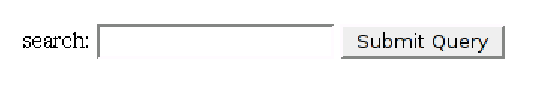
\epsfig{file=webclient}
\caption{Web-Client Screenshot}
\label{webclient}
\end{figure}

Als interessante Erweiterung, bot sich hier allerdings ein einfacher Javascript-Link an, der, als Bookmark in den eigenen Browser eingef"ugt, die Nachteile des Web-Clients zum Teil ausr"aumt:

\begin{verbatim}
javascript:location.href='http://serverurl/addpage.pl?
url='+encodeURIComponent(location.href)
\end{verbatim}

Mit diesem einfachen Link, kann das l"astige Kopieren umgangen werden, indem "uber Javascript die URL der aktuell im eigenen Browser angezeigten Seite, durch einen einfachen Click auf diesen Bookmark, direkt an den TeamFound-Server gesendet wird. (Beispiel ist f"ur Milestone 1)

\subsection{Implementation}
Die \textit{extrem einfache} Implementation des Web-Clients f"ur eine Suchanfrage entsprechend Milestone 2 sieht wie folgt aus:
\begin{verbatim}
<form action="serverurl">
	search: <input type="text" name="keyword">
	<input type="hidden" name="want" value="html">
	<input type="hidden" name="version" value="2">
	<input type="hidden" name="command" value="search">
	<input type="submit">
</form>
\end{verbatim}
Bei dem Design der TeamFound-Interfaces war diese M"oglichkeit der HTML-Formulare die entscheidende Grundlage. Alle Anfragen an den Server k"onnen mit HTML-Formularen ohne Zus"atze (wie Javascript, Applets, Extensions, etc.) generiert werden.

\section{Firefox-Toolbar}
Der Mozilla Firefox l"asst sich durch sogenannte \textit{Extensions} sehr einfach erweitern. Als grundlegende Techniken werden daf"ur XUL (XML User Interface Language) und Javascript ben"otigt. Desweiteren gibt es eine exakt vordefinierte Verzeichnisstruktur sowie eine Beschreibungs-Datei (\texttt{install.rdf}) im RDF (Resource Description Framework) Format, umd die Erweiterung automatisiert installierbar in Firefox-Browsern zu machen.

\begin{figure}
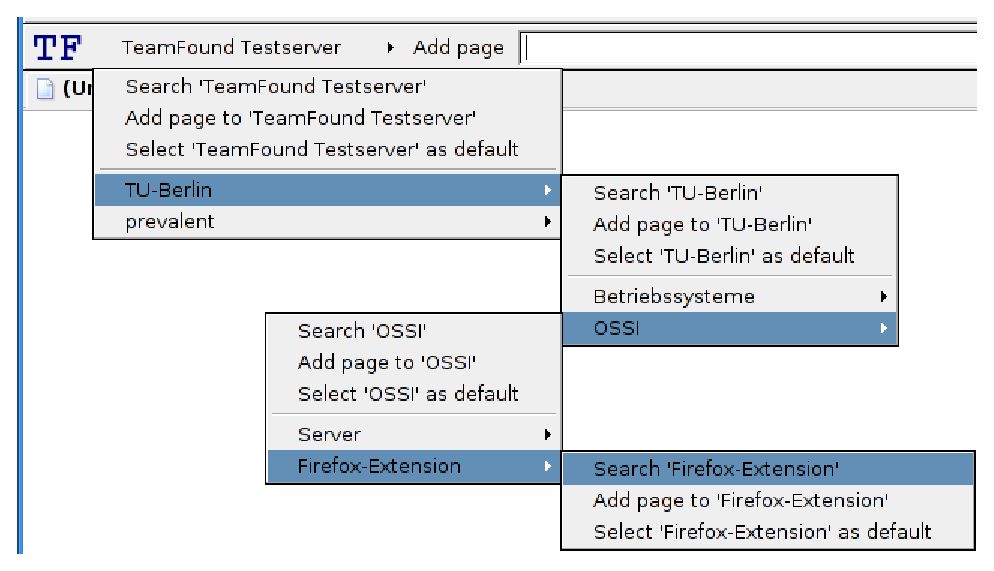
\epsfig{file=ffextension-kategorien}
\caption{Firefox-Toolbar mit Kategorien-Baum (v0.8, Milestone 2)}
\label{fftoolbar}
\end{figure}

\begin{figure}
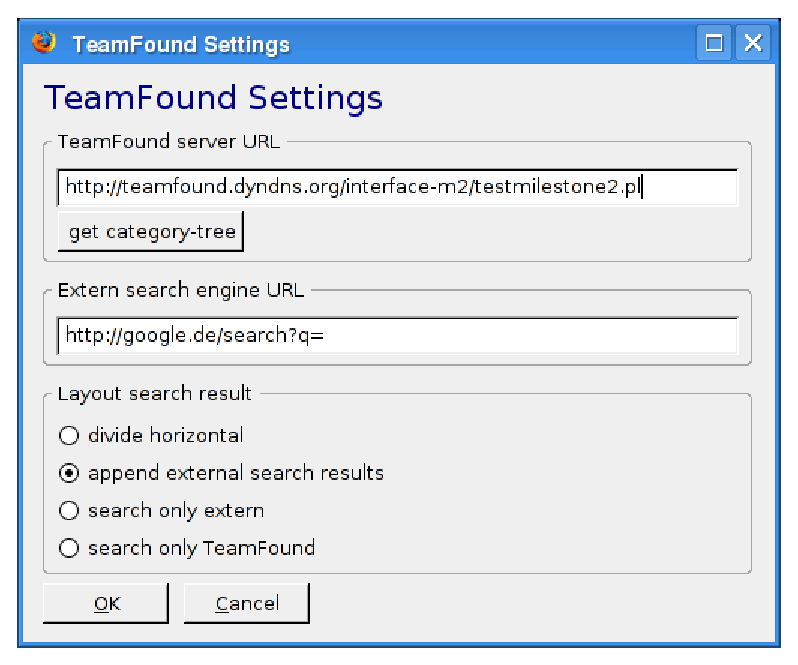
\epsfig{file=ffextension-settings}
\caption{Firefox-Toolbar Settings Dialog (v0.8, Milestone 2)}
\label{fftoolbar}
\end{figure}

\subsection{Dateien}
Die Verzeichnisstruktur der TeamFound Firefox Extension sowie alle enthaltenen Dateien sind:
\begin{verbatim}
chrome.manifest
install.rdf

content/
- overlay.js  
- overlay.xul  
- settings.js  
- settings.xul

defaults/
- preferences/
  - settings.js

skin/
- icon.png  
- logo_tf_32x32.png  
- overlay.css  
- search_h.html  
- search_v.html  
- xmlstyle.css
\end{verbatim}

Die eigentliche Funktionalit"at steckt dabei in dem Unterverzeichnis content:
\begin{description}
\item[overlay.xul] Definiert das Aussehen der Toolbar
\item[overlay.js] Definiert die Funktionalit"at der Toolbar
\item[settings.xul] Definiert das Aussehen des Einstellungen-Dialogs
\item[settings.js] Definiert die Funktionalit"at des Einstellungen-Dialogs
\end{description}

\begin{figure}
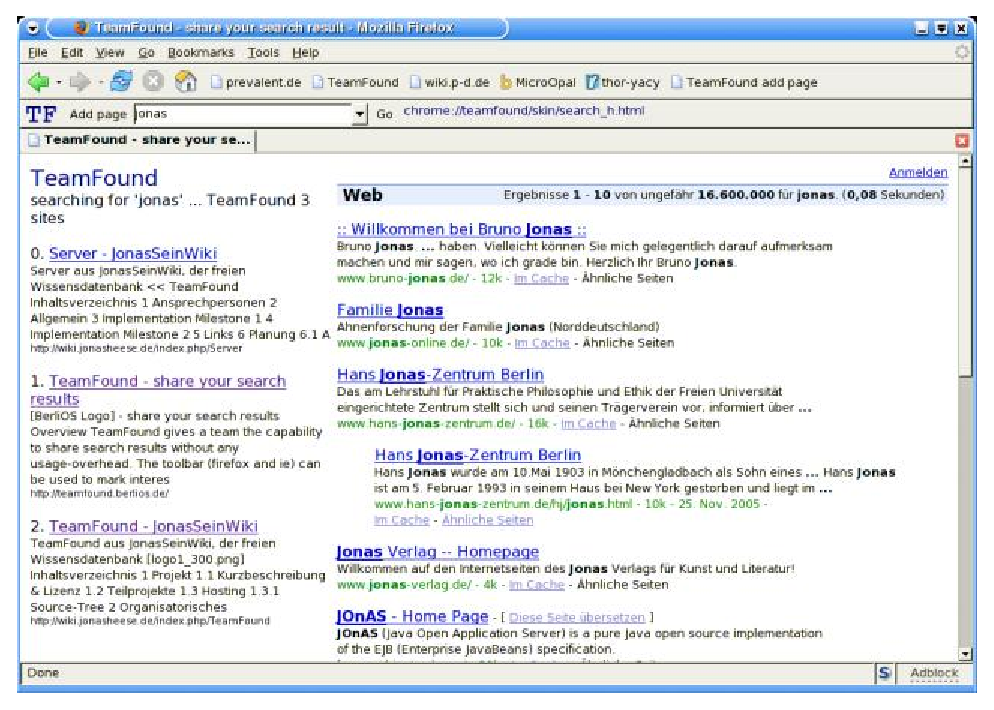
\epsfig{file=screenshot-search-server-0.1-firefox-toolbar-0.4.eps}
\caption{Firefox-Toolbar Suchergebnis (v0.4, Milestone 1)}
\label{fftoolbarsuchergebnis}
\end{figure}

\subsection{Changelog}
Das originale Changelog\footnote{\texttt{http://teamfound.berlios.de/\#firefoxchangelog0.7}} (in englischer Sprache):
\paragraph{Firefox \& Flock toolbar 0.7 (07-DEC-2005)}
\begin{itemize}
\item Bug-Fix: Add-Button actually works now
\item Label with current URL removed (though we are not going to replace the location-bar)
\item Compatibility with Flock browser tested and added to install.rdf
\end{itemize}

\paragraph{Firefox toolbar 0.6 (30-NOV-2005)}

\begin{itemize}
\item Input-field now behaves the same like the normal Firefox locationbar (including history popup) when urls are typed. Soon this can replace the Firefox locationbar and the Firefox searchbar with only one input-field ;-)
\item Settings-Dialog allows to give custom external search engines
\item Settings-Dialog allows to only search external, only search TeamFound or search both at once
\end{itemize}

\paragraph{Firefox toolbar 0.5 (28-NOV-2005)}

\begin{itemize}
\item Google search results are actually working now, including further results
\item Compatible with Firefox 1.5 release candidates
\end{itemize}

\paragraph{Firefox toolbar 0.4 (27-NOV-2005)}

\begin{itemize}
\item Clicking on TF-Icon opens preferences dialog, here you can setup your TeamFound server url and choose between two search result layouts
\item Add page - Adds the current page to the TeamFound-Index.
\item text field - Here you can enter search words or urls. The toolbar tries to automatically figure out what you meant and though will either search or just visit the given url.
\item current url - The current url is always displayed at the end of the toolbar, though not overwriting your current search words.
\end{itemize}

\paragraph{Firefox toolbar 0.3 (24-NOV-2005)}

\begin{itemize}
\item adds search at extern search-engine
\item shows google and teamfound search-results in same window
\end{itemize}

\paragraph{Firefox toolbar 0.2 (22-NOV-2005)}

\begin{itemize}
\item first release at berlios.de
\item available as .xpi
\end{itemize}

\paragraph{Firefox toolbar 0.1 (19-NOV-2005)}

\begin{itemize}
\item initial release
\end{itemize}

\section{Internet Explorer-Toolbar}

Auch beim Internet Explorer stand zun�chst die Frage wie dieser �berhaupt zu erweitern ist. 
Google und Yahoo haben mit ihren Toolbar's vorgemacht das es geht, nur das wie war zu l�sen.

Erste Anlaufstelle um der Probleml�sung n�her zu kommen 
war CodeProject (www.codeproject.com). 
Mit 2,8 Mio Mitgliedern ist sie die gr��te Community Seite f�r die Windows Entwicklung. 
Eine Suche nach ``IE Toolbar'' f�hrte zu einer .NET basierten Bibliothek 
f�r die Entwicklung von BandObjects, also Band Objekten (http://www.codeproject.com/csharp/dotnetbandobjects.asp).
Das mitgelieferte Beispiel funktionierte auf Anhieb 
und es wurde begonnen die Extension zu implementieren.

\subsection{Custom Explorer Bars, Tool Bands, and Desk Bands}

Es gibt verschiedene M�glichkeiten eigene Komponenten in den Internet Explorer zu integrieren. 
Im folgenden werden einige Konzepte vorgestellt.

\paragraph{Explorer Bars}

Ein zentrales Konzept zur Erweiterung des Internet Explorers, sind Explorer Bars. 
Explorer Bars sind Teilbereiche der Oberfl�che des Explorers, 
welche nicht zur Renderfl�che der HTML Seite geh�ren.
Explorer Bars wurden erstmalig mit dem Internet Explorer 4.0 eingef�hrt 
und bieten eine sehr flexible M�glichkeit den Explorer zu erweitern. 
Derzeit werden Funktionen wie Favorieten und die Suche innerhalb einer 
Explorer Bar dargestellt. Die Darstellung von Explorer Bars kann entweder Horizontal 
oder Vertikal erfolgen und sie werden �ber den Menu Ansicht -> Explorerleisten ein- und ausgeblendet.

\paragraph{Tool Bands}

Die Werkzeugleiste des Internet Explorers ist eine sogenannte ``Rebar'', 
also ein Container der wiederum mehrere Werkzeugleisten enthalten kann. 
Diese Werkzeugleisten werden Toolbands genannt. Erstmalig wurde das Konzept 
mit dem Internet Explorer 5.0 eingef�hrt um die Radio Leiste zu realisieren. 
Mittlerweile gibt es verschiedene Toolbands wie die Adressleiste und auch 
Fremdanbieter wie Google und Yahoo nutzen das Konzept.

\paragraph{Deskbands}

Diese Komponenten verfolgen den selben Ansatz, haben aber prim�r nichts mit dem Internet 
Explorer zu tun. Sie dienen dazu den Desktop um weitere Leisten zu erweitern. 
Ber�hmtester Vertreter dieser Kategorie ist die Adressleiste. 
Sie kann ausser im Explorer und Internet Explorer auch in der Taskleiste erscheinen.

\subsection{Entwicklung der Band Objekte}

Die Entwicklung dieser Komponenten basiert, wie ein sehr gro�er Teil der 
Windowsentwicklung auf COM. Das Component Objekt Model von Microsoft 
ist eines der �ltesten Komponentensysteme und bildet Zusammen mit dem 
Windows API die Grundlage f�r die Entwicklung von Windowssoftware.

\subsection{COM, Schnittstellen, Klassen, Registry}

Im folgende soll ein kurzer �berblick �ber COM gegeben werden, 
der die Schritte auf dem Weg zu Entwicklung der Band Objects erkl�rt.

\paragraph{COM Schnittstellen}

Zentrales Konzept von COM ist das Interface. In der COM Terminologie
 ist eine Schnittstelle, eine nach der COM Spezifikation aufgebauten, 
 Struktur mit Platzhaltern f�r Funktionszeiger. 
Diese Erkl�rung macht bereits deutlich auf welchem Level COM 
urspr�nglich definiert worden ist.
Schnittstellen k�nnen von Komponenten erfragt werden, und anschlie�end �ber 
die Methodenzeiger entsprechende Funktionen aufgerufen werden. 
In einer einfachen - praktisch puren - COM Application muss man das 
Aussehen der Schnittstellen genau kennen. Sp�ter kam ein Feature mit dem 
Namen ``OLE Automatisierung'' hinzu, welches �hnliche Konzepte wie Java Reflection bietet.
Jede Schnittstelle wird eindeutig �ber einen GUID - Global Unique Identifier - indentifiziert.
  
\paragraph{COM Komponenten}

Eine Komponente in der COM Terminologie ist eine abgeschlosse bin�re Einheit, 
welche Funktionalit�t �ber eine Schnittstelle bereitstellt. 
Komponenten sind also in Programmen (Executables) oder Bibliotheken (Dynamic Link Libraries) enthalten.

\paragraph{Registry}

Normalerweise, auch wenn das problemlos m�glich w�re, 
wird eine COM Bibliothek nicht direkt referenziert und geladen. 
Stattdessen nutz man Funktionen der COM API um eine Instanz einer Komponente mit einer 
bestimmten Schnittstelle zu erhalten. Dazu �bergibt man der Funktion die GUID der 
Schnittstelle welche man nutzen m�chte. Diese Funktion bem�ht die Windows Registry 
um die Bibliothek zu finden in der die Komponente mit der Schnittstelle implementiert ist, 
l�dt diese, erzeugt die Komponente und gibt die Schnittstelle zur�ck.
Damit das funktioniert, ist jede COM Komponente vor ihrer Benutzung in der Registry einzutragen.

\subsection{Band Objekte und COM}

Alle Band Objekte sind wiederum COM Komponenten, welche bestimmte Schnittstellen 
implementieren m�ssen. Diese Schnittstellen werden vom Internet Explorer erwartet und abgefragt. 
F�r die Entwicklung von Band Objekten m�ssen in jedem Fall die folgenden Schnittstellen implementiert werden:

\paragraph{IUnknown}

Das ist die Basisschnittstelle welche jedes COM Objekt implementieren muss. 
Sie bietet Funktionen zum Abrufen weiterer Schnittstellen sowie zur Referenzz�hlung.

\paragraph{IClassFactory}

Bietet Funktionen zum Erzeugen neuer Instanzen von COM Klassen.

\paragraph{IDeskBand}

Das ist die Basisschnittstelle f�r alle Band Objekte. IDeskBand erbt von 
IDockingWindow welches wiederum von IOleWindow erbt. Anhand der Namen der 
Schnittstellen lassen sich ungef�hr die Funktionen ableiten.
IOleWindow liefert das Fenster (jedes Element in Windows ist ein Fenster) 
an sich, IDockingWindow sorgt f�r das Anzeigen und Deaktivieren und 
IDeskBand liefert Informationen �ber das Band Objekt an sich.

Mit Hilfe von GetBandInfo kann der Internet Explorer ermitteln wie 
die Leiste heist, wie sie dargestellt werden soll und welche Gr��en sie haben darf.

\paragraph{IObjectWithSite}

�ber diese Schnisttelle hat man die M�glichkeit mit dem Container 
- also mit dem Internet Explorer zum Beispiel - des Band Objektes zu 
kommunizieren. Der Internet Explorer ist selbst ebenfalls ein COM Objekt 
welches diverse Schnittstellen implementiert. �ber die SetSite Funktion 
weist er dem Band Objekt die eigene IUnknown Schnittstelle zu.

\paragraph{IPersistStream}

Diese Schnittstelle wird vom Container verwendet um den Zustand des Band 
Objekts zu speichern oder zu laden. Das Band Objekt implementiert diese 
Schnittstelle um sich selbst in den �bergebenen Stream zu serialiasieren oder zu deserialisieren

Daneben gibt es noch einige weitere Schnittstellen z.B. f�r Benutzereingaben, 
auf welche hier jedoch nicht n�her eingegangen werden soll.

\subsection{Registrierung der Band Objekte}

Jedes Band Objekt muss wie bereits erw�hnt, als COM Objekt registriert werden. 
Dar�ber hinaus muss dem Internet Explorer nocht mitgeteilt werden, das er eine 
Toolleiste zur Verf�gung hat. Dies geschieht ebenfalls �ber einen Eintrag in der Windows Registry.

\subsection{Die BandObject Library}

Alles was im Abschnitt COM und Band Object Entwicklung beschrieben worden ist, 
nimmt einem die Band Objekt Library ab. Der ganze ``schmuzige'' COM Teil wird durch 
eine CSharp Klasse gekapselt welche von UserControll erbt und all die Schnittstellen implementiert. 
Was dem Entwickler der Toolbar bleibt ist eine Klasse zu erstellen 
welche von der BandObject erbt. Da BandObject selber von UserControl 
erbt, steht einem auch der visuelle Designer zum erstellen der Toolbar zur Verf�gung.
Die Funktionalit�t der Toolbar kann also bequem in CSharp erfolgen.

\subsection{Teamfound Internet Explorer Toolbar}

\paragraph{Entwicklung}


Installation

F�r die Installation auf einem Client PC kopiert man alle im Paket enthaltenen Quellen in einen Ordner.
Die Toolbar l�sst dann einfach mit dem Install.cmd installieren. Im wesentlichen passiert dabei folgendes:

Die Bibliotheken BandObject.dll und Teamfound.IE.dll werden als COM Objekt registriert und im globalen Assembly Cache registriert. 

Alle anderen Bibliotheken werden ebenfalls im globalen Assemblycache registriert.





\chapter{Projektverlauf}
\section{Organisation und Kommunikation by Jonas}

Das Teamfound-Projekt hat gleich mit zwei sehr starken Belastungen zu k�mpfen, einerseits ist es ein Open Source Projekt und kann zwar auf ordentliche Werkzeuge wie Revisionsverwaltung und Mailinglisten zur�ckgreifen, lebt jedoch von lockerer Organisation und der weitgehend freiwilligen Mitarbeit aller Beteiligten, andererseits ist es prim�r immernoch ein Projekt an der Universit�t und hat damit mit den ganz normalen Problemen solcher Projekte zu k�mpfen. Dies schliesst inbesondere den ganz eigenen Arbeitsablauf in derartigen Projekten ein, also mehr Aktivit�t, je n�her der Abgabetermin f�r diesen Bericht r�ckt.

Anders als im letzten Semester gab es dieses mal keine regelm��igen Treffen. Abgesehen von einem Starttreffen, bei dem vorallem Ideen f�r Erweiterungen und Bugs ausgetauscht wurden und einem Treffen kurz vor Schluss, in welchem die noch zahlreichen offenen Baustellen besprochen wurden, gab es kein Treffen von allen beteiligten. Benutzt wurde daher, wie auch im letzten Semester schon, die Mailingliste des Projektes (teamfound-development �t lists.berlios.de), um sich auszutauschen und Ideen und vorgehensweisen zu besprechen. Weitere Werkzeuge, wie sie Berlios anbietet, darunter Feature- und Bugtracker, wurden wohl auch aufgrudn des geringen nutzens f�r ein derart kleines Projekt noch nicht benutzt. Gegen Ende des Projektes sind auch die ungeplanten treffen im inoffiziellen Projekt-IRC-Channel (\#teamfound - quakenet) h�ufiger und bekannt f�r deren Produktivit�t geworden.
\subsection{Fazit: Probleme wachsender Projekte}

Teamfound besteht mittlerweile aus einer Menge Code, so sind alleine im Server mittlerweile an die einhundert Klassen mit vielen tausend Zeilen Code implementiert. In diesem Semester sind ausserdem viele Funktionen hinzugekommen, so das sich die Aktionsimplementierungen im Server fast verdoppelt haben. Es zeigt sich nun das die bisherige Architektur kaum mehr geeigent ist um mit den Anforderungen klarzukommen, so sind die zentralen Punkte im Server, n�mlich das Servlet, welches Requests entgegennimmt, validiert udn an den Controller weiterleitet, sowie dieser Controller, der die eigentliche Nutzlast f�r die einzelnen Aktionen implementiert,v�llig �berlaufen.
In Zukunft wird es also immer wichtiger effektive Strukturen f�r diese wachsenden Anforderungen zu schaffen und zu dokumentieren. Klare Datenschnittstellen sind notwendig und bisher kaum umgesetzt, die Kapselung von Funktionalit�t ist eine Aufgabe, welche die Architektur des Teamfound-Servers noch einmal deutlich ver�ndern wird. Die Auslagerung von Code in einzelne Bibliotheken-gleiche Implementierungen, wie zB. mit dem Crawler geschehen, k�nnen eine M�glichkeit sein, besser wart- und testbaren Code zu schreiben und auch f�r eine sauberere Implementierung sorgen. 
\section{Projektverlauf by Jan}

W"ahrend des Semesters hat sich eigentlich garnichts zu diesem Projekt getan. Selbst Steffen habe ich irgendwann im Juli 2006 gefragt ob wir uns nicht mal wieder Treffen sollten. Am 23. August 2006 war es dann soweit, und wir haben gemeinsam "uber m"ogliche Erweiterungen und neue Features diskutiert. Prinzipiell kam dabei aber nichts rum, was nicht schon lange (seit 15. Mai 2006) im wiki unter Milestone 3 eingetragen war. Die dort genannten Features f"ur den Server entsprechen lustigerweise auch genau den jetzt implementierten: 
\begin{verbatim}
http://wiki.jonasheese.de/index.php/Milestones

Server 17:05, 15. Mai 2006 Kechel (->Milestone 3 (SS06) - Planung)

* XSL-Stylesheet anstelle von HTML-Antwort von Server 
  -> es wird immer in XML geantwortet
* Web-Admin-Interface
* Framebasierte Seiten unterst�tzen
* User-Management
* Zeichensaetze beachten
* Automatisches Updated der eingetragenen Seiten (alle x tage oder so) 
\end{verbatim}

Inwieweit das mit den Zeichens"atzen tats"achlich funktioniert weiss ich pers"onlich nicht, ich habe aber im Source-Code gesehen das Jonas irgendwas mit ''encoding'' und so gemacht hat.

Nach diesem Treffen passierte wiederum erstmal eine Woche lang garnichts.

Ich begann dann am 2. September in unserem wiki das Interface f"ur Milestone 3 (\texttt{http://wiki.jonasheese.de/index.php/Interface\_Milestone\_3}) zu spezifizieren. Dazu "uberlegten Martin und ich welche Funktionen denn f"ur die obigen Features ben"otigt w"urden, welche Parameter sinnvoll seien und wie die XML-Antwort aussehen k"onnte. Leider hat Jonas's Server immernoch als Datum den 1. Januar 1970, daher ist die History dieses Dokuments nicht so eindeutig zur"uckzuverfolgen. F"ur sehr verl"asslich halte ich aber die Angaben in unserem Logbuch (\texttt{http://wiki.jonasheese.de/index.php/Logbuch}). Jedenfalls ist diese \textit{Spezifikation}, ausgedruckt auf DIN A4 Papier, 12 Seiten lang, und wurde im weiteren Projektverlauf von allen Projektseiten wohl am h"aufigsten benutzt und erweitert. Die einzig andere, f"ur mich n"utzliche Seite im Wiki, war \texttt{Server Milestone 3}, da Martin hier die Datenbank Tabellen incl. der Spaltennamen und Fremdschl"ussel aufgef"uhrt hat.

Am 6. September war wieder ein gemeinsames Treffen, jedoch waren nur Steffen, Andreas und Ich anwesend. Nach etwa zwei Stunden palaber war auch das geschafft. Wir hatten zwar interessante Themen, jedoch nicht wirklich spezifisch "uber das TeamFound Projekt diskutiert. 

Nach diesen Vorbereitungen war ich eine Woche im Ausland, mit dem Bewusstsein da"s nur nach meiner R"uckkehr nur noch eine einzige Woche Zeit verbleiben w"urde um "uberhaupt etwas zu implementieren. Dementsprechend vermisste ich auch sehr die nicht vorhandene Aktivit"at auf unserer Mailingliste. Nicht eine einzige Mail bzgl. TeamFound erreichte mich in dieser Zeit.  

Zum Gl"uck hatte sich doch etwas getan. Jedenfalls hatte Martin viel am DBLayer gearbeitet, und somit die Infrastruktur f"ur unsere neuen Features stark vorangebracht. Auch Jonas arbeitete schon am Index und Crawler. Was genau da alles ver"andert wurde oder werden sollte weiss ich nicht, aber bis jetzt hatte ich auch noch keine einzige Zeile am Sever selber geschrieben und wusste dementsprechend wenig dar"uber.

Hand in Hand mit Martin begann ich dann am Server zu arbeiten, und ein Feature nach dem anderen zu Implementieren. Da wir Zimmernachbarn sind, war die Kommunikation sehr sehr einfach und produktiv. Ich musste einfach nur \textit{r"ubergehen} und sagen $``$\textit{Hey, schalt mal deinen Chat-Client an, ich hab da ne Frage.}$``$ "Uber die folgenden Tage lernte ich so sehr schnell mich im Server-Code zurechtzufinden. Nebenbei erstellte ich noch das Web-Interface und passte die Firefox-Toolbar an das neue Interface an (ca. eine Stunde FF-Toolbar). Das Web-Interface entwickelte sich genauso wie Martin und ich Funktionen im Server fertigstellten, und nutzten dieses auch immer sofort um die neuen Funktionen zu testen. Jonas hatte derweil den neuen Indexer und Crawler fertiggestellt. Nach ein paar Stunden Bugfixing von Martin war diese Komponente auch compilierf"ahig in inseren Code integriert. (Jonas hatte anscheinend Probleme mit seinem Internetzugang, und konnte daher bis jetzt seine "Anderungen nicht comitten. Es ergaben sich auch viele Merge-Konflikte durch diese Verz"ogerung..)

Gestern, zwei Tage vor Abgabetermin, hatten wir endlich alle Features, bis auf das L"oschen von Kategorien und das automatische Updaten der indizierten Seiten, fertiggestellt, und ich konnte einen "offentlichen Testserver aufsetzen (\texttt{http://teamfound.dyndns.org:8080/tf/tf}). Im Chat kl"arten wir mit Andreas auch die letzten Interface-Fragen f"ur seine IE Toolbar implementation. Bis dahin hatte ich null Ahnung ob Andreas "uberhaupt an seinem Teil des Projekts arbeitet. Wie sich herausstellte ist seine Toolbar jedoch inzwischen wesentlich weiter als \textit{meine}. Immerhin half ich ihm einen Fehler beim Einloggen zu l"osen, eine Funktion die in der FF-Toolbar noch v"ollig fehlt.

Danach erstellte ich ein neues Release v0.9 der FF-Toolbar auf berlios.de und passte unsere Projekt Web-Seite \texttt{http://teamfound.berlios.de} entsprechend an.

Heute, einen Tag vor Abgabe, h"orte ich soeben von Martin, da"s die Update-Funktionalit"at nun auch funktioniert (w"ahrend ich selber diesen Text hier schreibe). Es sieht also so aus als w"urde alles \textit{just in time} fertig werden :)\\


Als Fazit w"urde ich sagen, da"s besonders die Interface Spezifikation sehr sehr Hilfreich war, um die zu implementierenden Features genau festzulegen. Auch die v"ollig von mir getrennt abgelaufene Entwicklung der Internet Explorer Toolbar wurde sicherlich nur dadurch m"oglich.

Innerhalb des Servers fehlten mir eben diese gemeinsamen Strukturen. Wie ich in der letzten Woche gelernt habe gibt es zwar auch dort viele feste Vereinbarungen, jedoch habe ich erst jetzt, nach einer Woche intensiver Besch"aftigung damit, den groben "Uberblick dar"uber erhalten. Ich bin sicher da"s Martin und Jonas diesen "Uberblick schon immer hatten, aber ich vermisste eine kurze Beschreibung z.B. im wiki dazu doch sehr. 

Es f"allt auch auf das keinerlei Coding-Styles vereinbart wurden. Es war mir nicht m"oglich Funktionsnamen aufgrund eines festgelegten Schemas zu erraten oder \textit{schnell} zu finden. Meist hab ich einfach Martin gefragt, und er hat mir dann gesagt ob es die Funktion, die xyz tut, schon gibt, oder ob ich diese neu Implementieren muss.

Zum Schluss noch die Anmerkung, da"s unser manuelles Logfile im wiki praktisch nur von mir alleine geupdated wurde. Ich hab zwar Martin immer wieder mal dazu "uberreden k"onnen, auch einzutragen was er denn so gemacht hat, aber das Interesse daran war wohl bei niemandem sehr hoch. Mir pers"onlich hat das Log besonders f"ur diesen Projektbericht sehr geholfen, aber f"ur die eigentliche Projektentwicklung war es nicht notwendig. Dennoch finde ich es selber sehr sch"on den Projektverlauf so zur"uckverfolgen zu k"onnen.\\

So, jetzt bin ich selber gespannt ob wir heute noch den Server v0.3 released bekommen.\\

Jan





\chapter{Fazit \& Ausblick}

\section{Probleme wachsender Projekte}

Teamfoudn besteht mittlerweile aus einer Menge Code, so sind alleine im Server mittlerweile an die einhundert Klassen mit vielen tausend Zeilen Code implementiert. In diesem Semester sind ausserdem viele Funktionen hinzugekommen, so das sich die Aktionsimplementierungen im Server fast verdoppelt haben. Es zeigt sich nun das die bisherige Architektur kaum mehr geeigent ist um mit den Anforderungen klarzukommen, so sind die zentralen Punkte im Server, n�mlich das Servlet, welches Requests entgegennimmt, validiert udn an den Controller weiterleitet, sowie dieser Controller, der die eigentliche Nutzlast f�r die einzelnen Aktionen implementiert,v�llig �berlaufen.
In Zukunft wird es also immer wichtiger effektive Strukturen f�r diese wachsenden Anforderungen zu schaffen und zu dokumentieren. Klare Datenschnittstellen sind notwendig und bisher kaum umgesetzt, die Kapselung von Funktionalit�t ist eine Aufgabe, welche die Architektur des Teamfound-Servers noch einmal deutlich ver�ndern wird. Die Auslagerung von Code in einzelne Bibliotheken-gleiche Implementierungen, wie zB. mit dem Crawler geschehen, k�nnen eine M�glichkeit sein, besser wart- und testbaren Code zu schreiben und auch f�r eine sauberere Implementierung sorgen. 

\begin{appendix}
\chapter{Interface}
\section{Interface Milestone 2}
\label{interface2}
\subsection{Allgemein}
\subsubsection{Tests}
Zum Testen der Serverseitigen Interface-Implementation existiert folgende Webseite, die entsprechende Requests erstellen kann: 

\texttt{http://teamfound.berlios.de/test\_the\_server\_interface\_m2.html}
\\
\\
Zum Testen der Clientseitigen Interface-Implementation existiert folgendes Perl-Skript, welches den Parameter command auswertet und eine enstsprechende statische XML-Antwort zurueckgibt: 
\\
\texttt{http://teamfound.dyndns.org/interface-m2/testmilestone2.pl}
\\
Demo: 
\\
\texttt{http://teamfound.dyndns.org/interface-m2/testmilestone2.pl?command=getcategories}
\\
Das Skript liegt auch im SVN unter \texttt{teamfound/interface/milestone2/testmilestone2.pl}

\subsubsection{Alle Anfragen an den Server}

Alle Anfrage-Parameter werden in Form von HTTP GET oder POST Variablen �bertragen. Prinzipiell gibt es eine Unterscheidung, ob f"ur jedes Kommando eine eigene URL verwendet wird, oder ob das Kommando in Form einer weiteren HTTP-GET Variablen mit "ubertragen wird. Unsere Implementation des  Servers verwendet den zus"atzlichen HTTP-GET Parameter \texttt{command}. In diesem Interface haben wir aber beide M"oglichkeiten spezifiziert.

\begin{description}
\item[want=xml or html] Die zu erwartende Antwort soll in xml oder html-format sein (default soll html werden, da dann einfache Link-Clients m�glich sind) 

\item[version=2] Milestone-Version des Interfaces 

\item[command=search] Das Kommando das ausgef�hrt werden soll. Dieses Argument kann wegfallen wenn f�r jedes Kommando eine eigene, gleichnamige Anfrage-URL existiert. 
\end{description}

\subsubsection{HTML-Antwort}
Die Clients geben an ob Sie eine HTML oder eine XML Antwort erwarten.

Soll eine vollst�ndige HTML-Seite zur�ckgeben, die direkt im Browser angezeigt werden kann. Die Return-Values wie bei einer XML-Antwort m�ssen in diesem Fall nicht zur�ckgegeben werden, sondern der Text sollte gleich eine entsprechende Meldung beinhalten.

\subsubsection{XML-Antwort}
\begin{description}
\item[$<$response$>$] Umschliesst alle anderen xml-tags und gibt die XSD-Datei zum verifizieren der XML-Daten an 
\item[$<$interface-version$>$] Gibt immer die Interface-Version an, in der die Antwort des Servers formuliert wurde 
\item[$<$server$>$] Gibt Name und Versionsnummer des Servers an. Der Server der unter der URL https://developer.berlios.de/projects/teamfound entwickelt wird gibt den Namen "TeamFound" zur�ck. Clones d�rfen Ihren eigenen Namen nat�rlich frei w�hlen. 
\item[$<$addpage$>$ $<$search$>$ $<$addcategory$>$ $<$getcategories$>$] Diese Tags beinhalten die Antworten auf die gleichnamigen Anfragen an den Server. Pro Anfrage darf nur eines dieser Tags vorkommen. 
\item[$<$return-value$>$ $<$return-description$>$] Der Return-Value bzw. Fehler-Code falls etwas schiefging. Die Description wird nicht genauer spezifiziert, sollte aber semantisch mit dem aufgetretenen Fehler �bereinstimmen. 
\item[$<$project-counter$>$] Bei jeder �nderung des Kategorien-Baumes( soll der Server einen internen Z�hler um eins inkrementieren. Der aktuelle Wert soll bei jeder XML-Antwort mit �bertragen werden. (Dann weiss die Toolbar wann sie selber die Kategorien neu vom Server abfragen muss.)Jedes Projekt fuehrt einen Counter, somit muss der Client nur die fuer ihn intressanten B"aume beachten. 
\end{description}

\begin{verbatim}
<response xmlns:xsi="http://www.w3.org/2001/XMLSchema-instance"
xsi:noNamespaceSchemaLocation="teamfound-interface-milestone2.xsd">

 <interface-version>2</interface-version>

 <return-value>0</return-value>
 <return-description>OK</return-description>

 <project-counter>
   <project>
     <projectID>0</projectID>
     <count>3</count>
   </project>
   <project>
     <projectID>3</projectID>
     <count>5</count>
   </project>
 </project-counter>

 <category-counter>54</category-counter>

 <server>
  <name>TeamFound</name>
  <version>0.2</version>
 </server>

 <addpage>
 </addpage>

 <search>
 </search>

 <addcategory>
 </addcategory>

 <getcategories>
 </getcategories>
 
</response>
\end{verbatim}

\paragraph{Return Codes}

Die Return-Codes stehen immer in den Tags $<$return-value$>$xx$<$/return-value$>$. Die Description ist optional.

\begin{description}
\item[0] Alles ok 

\item[1] Fehler, konnte URL nicht finden 

\item[2] Ung�ltige Anfrage (Pflicht-Parameter fehlen oder haben die L�nge null) 

\item[3] Inkompatible Interface-Version (die Anfrage hat eine Interface-Version benutzt die der Server nicht unterst�tzt) 

\item[4] Kategorie existiert schon (beim hinzufuegen einer neuen Kategorie) 

\item[5] Kategorie nicht gefunden (beim suchen nach einer bestimmten Kategorie) 

\item[-1] Anderer Fehler 
\end{description}

Die Return-Descriptions sind frei w�hlbar, sollten aber dem Return-Code semantisch entsprechen ;-)


\subsection{Seite hinzuf�gen}
\subsubsection{Anfrage an Server}

\begin{description}
\item[command=addpage] Der Kommando-Name 

\item[addpage.pl] Der (default) Skriptname der die Anfrage entgegennimmt (dann f�llt das Argument command weg). 

\item[category=453] Die Kategorien-Nummer zu der der Link hinzugefuegt werden soll, in dieser Version nur genau eine oder keine. Wird keine Kategorie angegeben, so soll die Top-Kategorie genommen werden (also nicht gefunden werden wenn bei der Suche eine genauere Kategorie angegeben wird). 

\item[url=http://yy.org/blabla.html] Die zu indizierende url, das Protokoll ist mit anzugeben 
\end{description}

\subsubsection{XML Antwort}
xml oder html um �ber Erfolg oder Misserfolg zu berichten

Verwendet in der Antwort das XML-Tag: $<$addpage$>$
\begin{verbatim}
<response>

 <interface-version>2</interface-version>

 <return-value>0</return-value>
 <return-description>OK</return-description>

 <server>
  <name>TeamFound</name>
  <version>0.2</version>
 </server>

 <addpage>
  <url>http://blabla.html</url>
 </addpage>
 
</response>
\end{verbatim}

\subsubsection{HTML Antwort}
siehe Allgemeines zu HTML-Antworten


\subsection{Suchen}
\subsubsection{Anfrage an Server}
\begin{description}
\item[command=search] Der Kommando-Name 

\item[search.pl] Der (default) Skriptname der die Anfrage entgegennimmt (dann f�llt das Argument command weg). 
\item[keyword=zzz] Eine durch ' ' (space) getrennte Liste der Suchw�rter die alle vorkommen sollen (URL-Codiert mit ''\%20'' getrennt, also eine Suche nach auto und tv wird als keyword=auto\%20tv codiert). Dies beinhaltet eine serverseitig impliziete UND-Verkn�pfung aller Suchworte. Fehlt der Parameter so soll ein Fehler zur�ckgegeben werden. Die genaue Definition einer umfassenderen Suchanfragen-Sprache (wie OR, NOT etc.) ist noch festzulegen, wird aber auf spaetere Interface-Milestones verschoben. 

\item[category=5\&category=9\&category=15] Eine Liste aller Kategorien-IDs, jeweils immer wieder neu mit category= durch die die Suche gemacht werden soll. Fehlt der Paramater, so soll alles durchsucht werden. (Grund: HTML-Formulare machen dies bei Listen und ComboBoxen mit Mehrfachauswahl genau so). 
\end{description}

\subsubsection{XML Antwort}
Verwendet in der Antwort das XML-Tag: $<$search$>$

\begin{verbatim}
<response>

 <interface-version>2</interface-version>

 <return-value>0</return-value>
 <return-description>OK</return-description>

 <server>
  <name>TeamFound</name>
  <version>0.2</version>
 </server>

 <search>

  <keywords>
   <word>xxx</word>
   <word>yyy</word>
  </keywords>

  <result>

   <count>30</count>
   <offset>0</offset>

   <found>
    <url>http://xxx.html</url>
    <title>Der Titel der Seite</title>
    <incategory>5</incategory>
   </found>

   <found>
    <url>http://xxx.html</url>
    <title>Der Titel der Seite</title>
    <incategory>5</incategory>
   </found>

   <found>
    <url>http://xxx.html</url>
    <title>Der Titel der Seite</title>
    <incategory>5</incategory>
    <incategory>3</incategory>
    <incategory>7</incategory>
   </found>

  </result>
 </search>
 
</response>
\end{verbatim}
\begin{itemize}
\item Die Keywords sind zur Fehlerbehandlung alle nochmals mit anzugeben. 

\item Jeder gefundene Link wird in einem eingenen $<$found$>$ Block augegeben. 

\item Wurde kein Suchergebnis gefunden, so ist in $<$count$>$ die Anzahl 0 einzutragen, der Return-Code aber immernoch 0 (OK) wenn sonst alles ok war 
\end{itemize}

\subsubsection{HTML Antwort}
HTML-Seite mit URLs gefundener �bereinstimmungen

\subsection{Kategorien von Server abfragen}
\subsubsection{Anfrage an Server}

\begin{description}
\item[command=getcategories] Der Kommando-Name 
\item[getcategories.pl] Der (default) Skriptname der die Anfrage entgegennimmt (dann f�llt das Argument command weg). 
\item[projectID=5] Nummer des projekts f�r diese Anfrage 
\end{description}

\subsubsection{XML Antwort}
Verwendet in der Antwort das XML-Tag: $<$getcategories$>$
\begin{verbatim}
<response>

 <interface-version>2</interface-version>

 <return-value>0</return-value>
 <return-description>OK</return-description>

 <server>
  <name>TeamFound</name>
  <version>0.2</version>
 </server>

 <getcategories>
  <category>
   <name>name der kategorie</name>
   <description>laengere beschreibung</description>
   <id>0</id>
   <subcategories>
    <category>
     ...
    </category>
    <category>
     ...
    </category>
   </subcategories>
  </category>
 </getcategories>
 
</response>
\end{verbatim}

Hinweis: die Top-Kategorie hat immer die ID 0 (null) 

\subsubsection{HTML Antwort}
siehe Allgemeines zu HTML-Antworten

\subsection{Kategorie hinzuf�gen}
\subsubsection{Anfrage an Server}
\begin{description}
\item[command=addcategory] Der Kommando-Name 

\item[addcategory.pl] Der (default) Skriptname der die Anfrage entgegennimmt (dann f�llt das Argument command weg). 

\item[name=kategoriename] Den Namen den die neue Kategorie bekommen soll 

\item[subcategoryof=45] Die Kategorie der die neue Kategorie untergeordnet werden soll. Soll eine neue 1st-Level Kategorie erstellt werden ist hier 0 (null) anzugeben. 

\item[description] Eine etwas l�ngere Beschreibung der Kategorie (max. 255 Zeichen) 
\end{description}

\subsubsection{XML Antwort}
Verwendet in der Antwort das XML-Tag: $<$addcategory$>$
\begin{verbatim}
<response>

 <interface-version>2</interface-version>

 <return-value>0</return-value>
 <return-description>OK</return-description>

 <server>
  <name>TeamFound</name>
  <version>0.2</version>
 </server>

 <addcategory>
  <name>kategoriename</name>
  <gotid>53</gotid>
 </addcategory>
 
</response>
\end{verbatim}
\begin{itemize}
\item der neue Name
\item die ID die die neue Kategorie bekommen hat
\item name und gotid fallen weg wenn die kategorie schon existiert (return-value 4 - Kategorie existiert schon) oder die subcategoryof-id nicht existiert (return-value 5 - Kategorie nicht gefunden). 
\end{itemize}

\subsubsection{HTML Antwort}
siehe Allgemeine HTML-Antwort

\subsection{Alle Projekte auslesen}
\subsubsection{Anfrage an Server}
\begin{description}
\item[command=getprojects] Der Kommando-Name 
\item[addcategory.pl] Der (default) Skriptname der die Anfrage entgegennimmt (dann f�llt das Argument command weg). 
\end{description}

\subsubsection{XML Antwort}
Verwendet in der Antwort das XML-Tag: $<$projects$>$
\begin{verbatim}
<response>

 <interface-version>2</interface-version>

 <return-value>0</return-value>
 <return-description>OK</return-description>

 <server>
  <name>TeamFound</name>
  <version>0.2</version>
 </server>

 <projects>
   <project>
     <name>prjectname</name>
     <description>beschreibung</description>
     <id>7</id>
   </project>
   ...
 </project>
 
</response>
\end{verbatim}

\subsubsection{HTML Anwort}
siehe Allgemeine HTML-Antwort

\subsection{L�schen einer Kategorie}
Wird erst in Interface Milestone 3 implementiert werden. Es stellt sich die Frage was mit den in dieser Kategorie bereits befindlichen Links gemacht wird .. verschieben?

\chapter{Logbuch}
\section{Projekt Logbuch}
Dies ist ein Snapshot des Projekt-Logbuchs vom 17. April 2006. Die jeweils aktuelle Version kann unter \texttt{http://wiki.jonasheese.de/index.php/Logbuch} eingesehen werden.
\subsection{2006}

\subsection{April 2006}
\paragraph{17. April 2006}
\begin{itemize}
\item Firefox-Extension v0.8 released Kechel 20:07, 17. Apr 2006 (CEST) 
\end{itemize}

\paragraph{11. April 2006}
\begin{itemize}
\item Vortrag gehalten Kechel 21:46, 11. Apr 2006 (CEST) 
\end{itemize}

\paragraph{10. April 2006}
\begin{itemize}
\item Vortrag-Slides fertig Kechel 20:14, 10. Apr 2006 (CEST)
\item FF-Extension 0.8 beta fertig incl. default-Kategorie (reicht fuer Praesentation ;-) Kechel 20:14, 10. Apr 2006 (CEST) 
\end{itemize}

\paragraph{9. April 2006}
\begin{itemize}
\item Vortrag-Slides angefangen Kechel 20:14, 10. Apr 2006 (CEST)
\item FF-Extension 0.8 funktioniert schon ganz gut Kechel 20:14, 10. Apr 2006 (CEST) 
\end{itemize}

\paragraph{8. April 2006}
\begin{itemize}
\item Ausarbeitung praktisch fertig incl. Anhang, Lizenz und Index Kechel 20:14, 10. Apr 2006 (CEST) 
\end{itemize}

\paragraph{7. April 2006}
\begin{itemize}
\item Ausarbeitung Anhang Kechel 20:14, 10. Apr 2006 (CEST)
\item ff-toolbar kategorien von echtem server geht Kechel 20:14, 10. Apr 2006 (CEST) 
\end{itemize}

\paragraph{4. April 2006}

\begin{itemize}
\item Ausarbeitung weitergeschrieben, Interface und Protokoll Kechel 20:14, 10. Apr 2006 (CEST)
\item FF-Extension 0.8 weiterprogrammiert Kechel 20:14, 10. Apr 2006 (CEST) 
\end{itemize}

\paragraph{2. April 2006}

\begin{itemize}
\item Ausarbeitung angefangen Kechel 20:14, 10. Apr 2006 (CEST) 
\end{itemize}


\subsubsection{M"arz 2006}

\paragraph{31. Maerz 2006}
\begin{itemize}
\item FF Client kann kategorien, kategorien durchsuchen und auch seiten zu kategorien hinzufuegen, die Anzeige von Suchergebnissen laesst noch sehr zu wuenschen uebrig Kechel 20:14, 10. Apr 2006 (CEST) 
\end{itemize}

\paragraph{12. Maerz 2006}
\begin{itemize}
\item XML-Kategorien-Baum wird in FF-Extension korrekt angezeigt. Kechel 16:07, 12. M�r 2006 (CET) 
\end{itemize}

\subsubsection{Januar 2006}
\paragraph{22. Januar 2006}
\begin{itemize}
\item Diese Woche den DBLayer vorlaeufig beendet. Moddin 14:27, 22. Jan 2006 (CET)
\item DBerlaeuterung im Wiki. Moddin 14:27, 22. Jan 2006 (CET)
\item Vortrag im Wiki vorbereitet, Themenauflistung, konkrete Vorschlaege. Kechel 21:51, 22. Jan 2006 (CET) 
\end{itemize}

\paragraph{12. Januar 2006}

\begin{itemize}
\item FF-Toolbar erstellt ersten M2 request (getcategories), werted die XML-Antwort aus und zeigt die erste Kategorie als Menuepunkt an. Kechel 17:05, 12. Jan 2006 (CET)
\item Testscript fuer Clients Milestone 2 geschrieben (http://wiki.jonasheese.de/index.php/Interface\_Milestone\_2\#Tests) Kechel 13:55, 12. Jan 2006 (CET) 
\end{itemize}

\subsection{2005}
\subsubsection{Dezember 2005}
\paragraph{7. Dezember 2005}
\begin{itemize}
\item FF-Toolbar 0.7 released (bug-fix). Kechel 16:08, 7. Dez 2005 (CET)
\item Test-Seite fuer Server Interface Milestone 2 Implementation erstellt (http://teamfound.berlios.de/test\_the\_server\_interface\_m2.html). Kechel 20:09, 7. Dez 2005 (CET) 
\end{itemize}

\paragraph{6. Dezember 2005}
\begin{itemize}
\item Label mit aktueller URL aus FF-Toolbar entfernt. Kechel 18:48, 6. Dez 2005 (CET) 
\end{itemize}

\paragraph{5. Dezember 2005}
\begin{itemize}
\item Code Review von Martins Zeug, morgen m�ssen wir auf jedenfall die Architektur genauer festelegen, das wir kein Chaos produzieren. --Jonas 21:18, 5. Dez 2005 (CET) 
\end{itemize}

\paragraph{2. Dezember 2005}

\begin{itemize}
\item Toolbar jetzt auch ueber http://addons.mozilla.org verfuegbar. Kechel 19:22, 2. Dez 2005 (CET) 
\end{itemize}
\begin{verbatim}
TeamFound 0.6 - Approval Granted
Your item, TeamFound 0.6, has been reviewed by a 
Mozilla Update editor who took the following action:
Approval Granted

Please Note: It may take up to 30 minutes for your 
extension to be available for download.

Your item was tested by Chris Blore using Firefox 1.5 on Windows XP.
Editor's Comments:
Thanks for submitting
\end{verbatim}

\paragraph{1. Dezember 2005}
\begin{itemize}
\item Firefox-Toolbar ist jetzt auch eine Flock-Toolbar (also compatibel zum flock-browser http://www.flock.com). Kechel 19:13, 1. Dez 2005 (CET) 
\item Firefox-Toolbar ist jetzt auch eine Flock-Toolbar (also compatibel zum flock-browser http://www.flock.com). Kechel 19:13, 1. Dez 2005 (CET) 
\end{itemize}

\subsubsection{November 2005}
\paragraph{30. November 2005}

\begin{itemize}
\item Milestone 1 Version als Servlet gebastelt.Moddin 19:57, 30. Nov 2005 (CET)
\item Firefox toolbar 0.6 released. Kechel 23:54, 30. Nov 2005 (CET) 
\end{itemize}


\paragraph{29. November 2005}

\begin{itemize}
\item Gemeinsam Interface Milestone 2 verabschiedet. Kechel 15:23, 30. Nov 2005 (CET) 
\end{itemize}

\paragraph{28. November 2005}
\begin{itemize}
\item Firefox-Toolbar 0.5 released, google links funktionieren endlich (auch die weitere-ergebnisse-links). In CustomizeGoogle Malingliste gefragt wie wir unsere extensions zur Kooperation bringen koennten. Kechel 16:15, 28. Nov 2005 (CET) 
\end{itemize}

\paragraph{27. November 2005}

\begin{itemize}
\item Toolbar bei addons.mozilla.org hochgeladen, waiting for review and aproval. Kechel 23:16, 27. Nov 2005 (CET)
\item Firefox-Toolbar v0.4 ist fertig, asyncrones laden der TeamFound und google ergebnisse, sowie eingegebene urls werden nicht gesucht sondern direkt angesprungen. Kechel 15:08, 27. Nov 2005 (CET) 
\end{itemize}

\paragraph{26. November 2005}

\begin{itemize}
\item Firefox-Toolbar hat nun auch einen Einstellungen-Dialog fuer die Server-Adresse. Kechel 22:49, 26. Nov 2005 (CET) 
\end{itemize}

\paragraph{25. November 2005}
\begin{itemize}
\item XSD-Datei zum verifizieren der XLM-Daten nach Interface Milestone 2 erzeugt. Kechel 18:12, 25. Nov 2005 (CET) 
\end{itemize}

\paragraph{24. November 2005}

\begin{itemize}
\item Firefox-Toolbar sucht jetzt auch selber noch bei google und zeigt die Ergebnisse von TeamFound und google nebeneinander an. Version 0.3 der Toolbar released. Kechel 22:54, 24. Nov 2005 (CET) 
\end{itemize}

\paragraph{23. November 2005}

\begin{itemize}
\item Am ServerProgramm ein paar Verbesserungen vorgenommen hinsichtlich der Performance
\item Script und java so erweitert das adding bei gesetztem lock wartet(sehr simple variante) Moddin 21:17, 23. Nov 2005 (CET)
\item Server-Release 0.1 auf Berlios geladen, kleine install.txt hinzugefuegt, $<$category-counter$>$ zu Interface Milestone 2 hinzugefuegt. Kechel 16:23, 23. Nov 2005 (CET)
\item Web-Client geschrieben (einfaches HTML-Formular zum suchen, und link zum adden neuer seiten). Kechel 20:21, 23. Nov 2005 (CET) 
\end{itemize}

\paragraph{22. November 2005}
\begin{itemize}
\item Firefox-Extension 0.2 xpi-file erstellt und als erstes file auf berlios released, installations-anleitung angepasst und link auf end-user homepage gesetzt. Kechel 19:46, 22. Nov 2005 (CET)
\item Interface Milestone 2 spezifiziert (als Vorschlag, aber schon sehr weit ausgearbeitet!) Kechel 21:59, 22. Nov 2005 (CET) 
\end{itemize}

\paragraph{21. November 2005}

\begin{itemize}
\item An den Server Interna gearbeitet um Milestone 1. naeherzukommen (Files sind im svn, fortlaufenden Index von Seiten kann gebaut und durchsucht werden) Moddin 21:05, 21. Nov 2005 (CET) 
\end{itemize}

\paragraph{19. November 2005}

\begin{itemize}
\item Firefox-Toolbar ist in version 0.1 fertig und einsatzbereit. Es koennen Seiten hinzugefuegt werden und diese wieder durchsucht werden. Der Server funktioniert ebenfalls in einer ersten Version bei uns lokal auf einem Rechner. Der Index wird jedoch bei jeder neu hinzugefuegten seite komplett ueberschrieben, so dass immer nur die zuletzt hinzugefuege Seite durchsucht wird ;-) Kechel 20:13, 19. Nov 2005 (CET)
\item Installations-Anleitung fuer Server-Milestone 1 geschrieben. Kechel 20:39, 19. Nov 2005 (CET)
\item Installations-Anleitung und kleine Doku fuer Firefox-Toolbar Milestone 1 erstellt. Kechel 22:48, 19. Nov 2005 (CET)
\item Logo auf http://teamfound.berlios.de upgeloaded und in Pr�sentation vorgestellt. Kechel 23:07, 19. Nov 2005 (CET)
\item Icon in Firefox-Toolbar eingebaut und screenshot ins wiki getan damit endlich mal etwas optisch anspruchsvolles im wiki ist ;-) Kechel 00:41, 20. Nov 2005 (CET) 
\end{itemize}

\paragraph{17. November 2005}
\begin{itemize}
\item Erste Server-Perl Skripte in SVN getan und in Server entsprechende Beschreibung eingefuegt. Kechel 15:59, 17. Nov 2005 (CET) 
\end{itemize}

\paragraph{15. November 2005}
\begin{itemize}
\item Interface-Spezifikation f�r Milestone 1 fertig. Kechel 11:03, 15. Nov 2005 (CET)
\item Erste Server-Perl Scripte erstellt. Jan \& Moddin 
\end{itemize}

\paragraph{12. November 2005}
\begin{itemize}
\item kleiner Testlauf mit Lucene-Demo bei mir ... 270 MB hat ungefaehr 3 min gebraucht zum index erstellen und nahm 14 MB ein. Ausserdem haben sie auch nen HTMLParser in der Demo aber nur fuer reine HTML-Files ... alles andere wird dann nicht mit index versehen, aber immerhin fuer uns schon sehr nuetzlich. Moddin 15:04, 12. Nov 2005 (CET) 
\end{itemize}

\paragraph{09. November 2005}

\begin{itemize}
\item Mailingliste teamfound-development@lists.berlios.de eingerichtet und entsprechende links auf diesem wiki plaziert. Kechel 15:25, 9. Nov 2005 (CET)
\item Erster SVN-Checkout sowie erste Firefox-Toolbar upgeloaded. Kechel 16:06, 9. Nov 2005 (CET) 
\end{itemize}

\paragraph{08. November 2005}
\begin{itemize}
\item Erste eigene Firefox-Extension erstellt die auch funktioniert (Menu-Item 'TeamFound' der beim anklicken eine MsgBox ausgibt ;-) Kechel 23:25, 8. Nov 2005 (CET) 
\end{itemize}

\paragraph{07. November 2005}
\begin{itemize}
\item Nach nutzbaren tools fuer den Server gesucht und alles was ich so gefunden habe ins Wiki unter Server geschrieben.Moddin 16:43, 7. Nov 2005 (CET)
\item Nach Informationen zum IE Plugin gesucht und alles unter Toolbar als Extension f�r Internet Explorer eingetragen.Andreas 22:34, 7. Nov 2005 (CET)
\item Erste Firefox-Extension versucht zu programmieren .. naja, und zum ersten mal von XUL gehoert ;-) Aber dafuer hat die HelloWorld-Extension gleich funktioniert! Kechel 23:45, 7. Nov 2005 (CET) 
\end{itemize}

\paragraph{03. November 2005}

\begin{itemize}
\item berlios-Services sind inzwischen aktiv, also shell login geht, die domain teamfound.berlios.de ist erreichbar und ich habe auch gleich mal einen minimalen content aufgesetzt. Kechel 14:01, 3. Nov 2005 (CET) 
\item Projekt bei berlios.de wurde approved. Projekt ein bisschen eingerichtet, wichtige infos auf wiki uebertragen. Kechel 11:51, 3. Nov 2005 (CET) 
\item Projekt teamfound auf berlios.de beantragt. Kechel 00:27, 3. Nov 2005 (CET) 
\end{itemize}

\paragraph{02. November 2005}

\begin{itemize}
\item TeamFound Wiki-Seite grunds�tzlich strukturiert, Teilprojekte angelegt und �berall mal einen Anfang formuliert. Kechel 23:00, 2. Nov 2005 (CET) 
\end{itemize}

\paragraph{01. November 2005}

\begin{itemize}
\item Nachtrag: Gemeinsames Treffen an Uni, Festlegung der Projekte, und verteilung der Projektmitglieder (so kamen wir 4 erstmals zu diesem Projekt zusammen). Kechel 23:00, 2. Nov 2005 (CET) 
\end{itemize}


\section{Firefox Toolbar Changelog}
\label{changelog}
Das originale \index{Changelog}Changelog\footnote{\texttt{http://teamfound.berlios.de/\#firefoxchangelog0.7}} (in englischer Sprache):
\subsection{2006}
Bisher noch kein neues Release in 2006. Die version 0.8 ist zwar bereits eine vollst"andige Imlementation nach Mileston 2, funktioniert aber noch nicht stabil genug um diese als neues Release freizugeben.
\subsection{2005}
\subsubsection{Firefox \& Flock toolbar 0.7 (07-DEC-2005)}
\begin{itemize}
\item Bug-Fix: Add-Button actually works now
\item Label with current URL removed (though we are not going to replace the location-bar)
\item Compatibility with Flock browser tested and added to install.rdf
\end{itemize}

\subsubsection{Firefox toolbar 0.6 (30-NOV-2005)}

\begin{itemize}
\item Input-field now behaves the same like the normal Firefox locationbar (including history popup) when urls are typed. Soon this can replace the Firefox locationbar and the Firefox searchbar with only one input-field ;-)
\item Settings-Dialog allows to give custom external search engines
\item Settings-Dialog allows to only search external, only search TeamFound or search both at once
\end{itemize}

\subsubsection{Firefox toolbar 0.5 (28-NOV-2005)}

\begin{itemize}
\item Google search results are actually working now, including further results
\item Compatible with Firefox 1.5 release candidates
\end{itemize}

\subsubsection{Firefox toolbar 0.4 (27-NOV-2005)}

\begin{itemize}
\item Clicking on TF-Icon opens preferences dialog, here you can setup your TeamFound server url and choose between two search result layouts
\item Add page - Adds the current page to the TeamFound-Index.
\item text field - Here you can enter search words or urls. The toolbar tries to automatically figure out what you meant and though will either search or just visit the given url.
\item current url - The current url is always displayed at the end of the toolbar, though not overwriting your current search words.
\end{itemize}

\subsubsection{Firefox toolbar 0.3 (24-NOV-2005)}

\begin{itemize}
\item adds search at extern search-engine
\item shows google and teamfound search-results in same window
\end{itemize}

\subsubsection{Firefox toolbar 0.2 (22-NOV-2005)}

\begin{itemize}
\item first release at berlios.de
\item available as .xpi
\end{itemize}

\subsubsection{Firefox toolbar 0.1 (19-NOV-2005)}

\begin{itemize}
\item initial release
\end{itemize}

\chapter{TeamFound Programm Lizenz}
TeamFound sowie alle enthaltenen Komponenten wie Source-Code, Binaries und Bilder stehen under der GNU General Public License (GPL) Version 2 oder h"oher. Eine Kopie der Lizenz liegt allen Source- und Bin"ar Versionen bei.\\
\\
\textbf{TeamFound - share your search results}\\
\textbf{Copyright \copyright 2005-2006 Jan Kechel, Martin Klink, Jonas Heese, Andreas Bachmann}\\
\\
This program is free software; you can redistribute it and/or
modify it under the terms of the GNU General Public License
as published by the Free Software Foundation; either version 2
of the License, or (at your option) any later version.
This program is distributed in the hope that it will be useful,
but WITHOUT ANY WARRANTY; without even the implied warranty of
MERCHANTABILITY or FITNESS FOR A PARTICULAR PURPOSE. See the
GNU General Public License for more details.
You should have received a copy of the GNU General Public License
along with this program; if not, write to the Free Software
Foundation, Inc., 51 Franklin Street, Fifth Floor, Boston, MA 02110-1301, USA.

\chapter{GNU Free Documentation License}
%\label{label_fdl}

 \begin{center}

       Version 1.2, November 2002


 Copyright \copyright 2000,2001,2002  Free Software Foundation, Inc.
 
 \bigskip
 
     51 Franklin St, Fifth Floor, Boston, MA  02110-1301  USA
  
 \bigskip
 
 Everyone is permitted to copy and distribute verbatim copies
 of this license document, but changing it is not allowed.
\end{center}


\begin{center}
{\bf\large Preamble}
\end{center}

The purpose of this License is to make a manual, textbook, or other
functional and useful document ''free'' in the sense of freedom: to
assure everyone the effective freedom to copy and redistribute it,
with or without modifying it, either commercially or noncommercially.
Secondarily, this License preserves for the author and publisher a way
to get credit for their work, while not being considered responsible
for modifications made by others.

This License is a kind of ''copyleft'', which means that derivative
works of the document must themselves be free in the same sense.  It
complements the GNU General Public License, which is a copyleft
license designed for free software.

We have designed this License in order to use it for manuals for free
software, because free software needs free documentation: a free
program should come with manuals providing the same freedoms that the
software does.  But this License is not limited to software manuals;
it can be used for any textual work, regardless of subject matter or
whether it is published as a printed book.  We recommend this License
principally for works whose purpose is instruction or reference.


\begin{center}
{\Large\bf 1. APPLICABILITY AND DEFINITIONS}
\addcontentsline{toc}{section}{1. APPLICABILITY AND DEFINITIONS}
\end{center}

This License applies to any manual or other work, in any medium, that
contains a notice placed by the copyright holder saying it can be
distributed under the terms of this License.  Such a notice grants a
world-wide, royalty-free license, unlimited in duration, to use that
work under the conditions stated herein.  The \textbf{''Document''}, below,
refers to any such manual or work.  Any member of the public is a
licensee, and is addressed as \textbf{''you''}.  You accept the license if you
copy, modify or distribute the work in a way requiring permission
under copyright law.

A \textbf{''Modified Version''} of the Document means any work containing the
Document or a portion of it, either copied verbatim, or with
modifications and/or translated into another language.

A \textbf{''Secondary Section''} is a named appendix or a front-matter section of
the Document that deals exclusively with the relationship of the
publishers or authors of the Document to the Document's overall subject
(or to related matters) and contains nothing that could fall directly
within that overall subject.  (Thus, if the Document is in part a
textbook of mathematics, a Secondary Section may not explain any
mathematics.)  The relationship could be a matter of historical
connection with the subject or with related matters, or of legal,
commercial, philosophical, ethical or political position regarding
them.

The \textbf{''Invariant Sections''} are certain Secondary Sections whose titles
are designated, as being those of Invariant Sections, in the notice
that says that the Document is released under this License.  If a
section does not fit the above definition of Secondary then it is not
allowed to be designated as Invariant.  The Document may contain zero
Invariant Sections.  If the Document does not identify any Invariant
Sections then there are none.

The \textbf{''Cover Texts''} are certain short passages of text that are listed,
as Front-Cover Texts or Back-Cover Texts, in the notice that says that
the Document is released under this License.  A Front-Cover Text may
be at most 5 words, and a Back-Cover Text may be at most 25 words.

A \textbf{''Transparent''} copy of the Document means a machine-readable copy,
represented in a format whose specification is available to the
general public, that is suitable for revising the document
straightforwardly with generic text editors or (for images composed of
pixels) generic paint programs or (for drawings) some widely available
drawing editor, and that is suitable for input to text formatters or
for automatic translation to a variety of formats suitable for input
to text formatters.  A copy made in an otherwise Transparent file
format whose markup, or absence of markup, has been arranged to thwart
or discourage subsequent modification by readers is not Transparent.
An image format is not Transparent if used for any substantial amount
of text.  A copy that is not ''Transparent'' is called \textbf{''Opaque''}.

Examples of suitable formats for Transparent copies include plain
ASCII without markup, Texinfo input format, LaTeX input format, SGML
or XML using a publicly available DTD, and standard-conforming simple
HTML, PostScript or PDF designed for human modification.  Examples of
transparent image formats include PNG, XCF and JPG.  Opaque formats
include proprietary formats that can be read and edited only by
proprietary word processors, SGML or XML for which the DTD and/or
processing tools are not generally available, and the
machine-generated HTML, PostScript or PDF produced by some word
processors for output purposes only.

The \textbf{''Title Page''} means, for a printed book, the title page itself,
plus such following pages as are needed to hold, legibly, the material
this License requires to appear in the title page.  For works in
formats which do not have any title page as such, ''Title Page'' means
the text near the most prominent appearance of the work's title,
preceding the beginning of the body of the text.

A section \textbf{''Entitled XYZ''} means a named subunit of the Document whose
title either is precisely XYZ or contains XYZ in parentheses following
text that translates XYZ in another language.  (Here XYZ stands for a
specific section name mentioned below, such as \textbf{''Acknowledgements''},
\textbf{''Dedications''}, \textbf{''Endorsements''}, or \textbf{''History''}.)  
To \textbf{''Preserve the Title''}
of such a section when you modify the Document means that it remains a
section ''Entitled XYZ'' according to this definition.

The Document may include Warranty Disclaimers next to the notice which
states that this License applies to the Document.  These Warranty
Disclaimers are considered to be included by reference in this
License, but only as regards disclaiming warranties: any other
implication that these Warranty Disclaimers may have is void and has
no effect on the meaning of this License.


\begin{center}
{\Large\bf 2. VERBATIM COPYING}
\addcontentsline{toc}{section}{2. VERBATIM COPYING}
\end{center}

You may copy and distribute the Document in any medium, either
commercially or noncommercially, provided that this License, the
copyright notices, and the license notice saying this License applies
to the Document are reproduced in all copies, and that you add no other
conditions whatsoever to those of this License.  You may not use
technical measures to obstruct or control the reading or further
copying of the copies you make or distribute.  However, you may accept
compensation in exchange for copies.  If you distribute a large enough
number of copies you must also follow the conditions in section 3.

You may also lend copies, under the same conditions stated above, and
you may publicly display copies.


\begin{center}
{\Large\bf 3. COPYING IN QUANTITY}
\addcontentsline{toc}{section}{3. COPYING IN QUANTITY}
\end{center}


If you publish printed copies (or copies in media that commonly have
printed covers) of the Document, numbering more than 100, and the
Document's license notice requires Cover Texts, you must enclose the
copies in covers that carry, clearly and legibly, all these Cover
Texts: Front-Cover Texts on the front cover, and Back-Cover Texts on
the back cover.  Both covers must also clearly and legibly identify
you as the publisher of these copies.  The front cover must present
the full title with all words of the title equally prominent and
visible.  You may add other material on the covers in addition.
Copying with changes limited to the covers, as long as they preserve
the title of the Document and satisfy these conditions, can be treated
as verbatim copying in other respects.

If the required texts for either cover are too voluminous to fit
legibly, you should put the first ones listed (as many as fit
reasonably) on the actual cover, and continue the rest onto adjacent
pages.

If you publish or distribute Opaque copies of the Document numbering
more than 100, you must either include a machine-readable Transparent
copy along with each Opaque copy, or state in or with each Opaque copy
a computer-network location from which the general network-using
public has access to download using public-standard network protocols
a complete Transparent copy of the Document, free of added material.
If you use the latter option, you must take reasonably prudent steps,
when you begin distribution of Opaque copies in quantity, to ensure
that this Transparent copy will remain thus accessible at the stated
location until at least one year after the last time you distribute an
Opaque copy (directly or through your agents or retailers) of that
edition to the public.

It is requested, but not required, that you contact the authors of the
Document well before redistributing any large number of copies, to give
them a chance to provide you with an updated version of the Document.


\begin{center}
{\Large\bf 4. MODIFICATIONS}
\addcontentsline{toc}{section}{4. MODIFICATIONS}
\end{center}

You may copy and distribute a Modified Version of the Document under
the conditions of sections 2 and 3 above, provided that you release
the Modified Version under precisely this License, with the Modified
Version filling the role of the Document, thus licensing distribution
and modification of the Modified Version to whoever possesses a copy
of it.  In addition, you must do these things in the Modified Version:

\begin{itemize}
\item[A.] 
   Use in the Title Page (and on the covers, if any) a title distinct
   from that of the Document, and from those of previous versions
   (which should, if there were any, be listed in the History section
   of the Document).  You may use the same title as a previous version
   if the original publisher of that version gives permission.
   
\item[B.]
   List on the Title Page, as authors, one or more persons or entities
   responsible for authorship of the modifications in the Modified
   Version, together with at least five of the principal authors of the
   Document (all of its principal authors, if it has fewer than five),
   unless they release you from this requirement.
   
\item[C.]
   State on the Title page the name of the publisher of the
   Modified Version, as the publisher.
   
\item[D.]
   Preserve all the copyright notices of the Document.
   
\item[E.]
   Add an appropriate copyright notice for your modifications
   adjacent to the other copyright notices.
   
\item[F.]
   Include, immediately after the copyright notices, a license notice
   giving the public permission to use the Modified Version under the
   terms of this License, in the form shown in the Addendum below.
   
\item[G.]
   Preserve in that license notice the full lists of Invariant Sections
   and required Cover Texts given in the Document's license notice.
   
\item[H.]
   Include an unaltered copy of this License.
   
\item[I.]
   Preserve the section Entitled ''History'', Preserve its Title, and add
   to it an item stating at least the title, year, new authors, and
   publisher of the Modified Version as given on the Title Page.  If
   there is no section Entitled ''History'' in the Document, create one
   stating the title, year, authors, and publisher of the Document as
   given on its Title Page, then add an item describing the Modified
   Version as stated in the previous sentence.
   
\item[J.]
   Preserve the network location, if any, given in the Document for
   public access to a Transparent copy of the Document, and likewise
   the network locations given in the Document for previous versions
   it was based on.  These may be placed in the ''History'' section.
   You may omit a network location for a work that was published at
   least four years before the Document itself, or if the original
   publisher of the version it refers to gives permission.
   
\item[K.]
   For any section Entitled ''Acknowledgements'' or ''Dedications'',
   Preserve the Title of the section, and preserve in the section all
   the substance and tone of each of the contributor acknowledgements
   and/or dedications given therein.
   
\item[L.]
   Preserve all the Invariant Sections of the Document,
   unaltered in their text and in their titles.  Section numbers
   or the equivalent are not considered part of the section titles.
   
\item[M.]
   Delete any section Entitled ''Endorsements''.  Such a section
   may not be included in the Modified Version.
   
\item[N.]
   Do not retitle any existing section to be Entitled ''Endorsements''
   or to conflict in title with any Invariant Section.
   
\item[O.]
   Preserve any Warranty Disclaimers.
\end{itemize}

If the Modified Version includes new front-matter sections or
appendices that qualify as Secondary Sections and contain no material
copied from the Document, you may at your option designate some or all
of these sections as invariant.  To do this, add their titles to the
list of Invariant Sections in the Modified Version's license notice.
These titles must be distinct from any other section titles.

You may add a section Entitled ''Endorsements'', provided it contains
nothing but endorsements of your Modified Version by various
parties--for example, statements of peer review or that the text has
been approved by an organization as the authoritative definition of a
standard.

You may add a passage of up to five words as a Front-Cover Text, and a
passage of up to 25 words as a Back-Cover Text, to the end of the list
of Cover Texts in the Modified Version.  Only one passage of
Front-Cover Text and one of Back-Cover Text may be added by (or
through arrangements made by) any one entity.  If the Document already
includes a cover text for the same cover, previously added by you or
by arrangement made by the same entity you are acting on behalf of,
you may not add another; but you may replace the old one, on explicit
permission from the previous publisher that added the old one.

The author(s) and publisher(s) of the Document do not by this License
give permission to use their names for publicity for or to assert or
imply endorsement of any Modified Version.


\begin{center}
{\Large\bf 5. COMBINING DOCUMENTS}
\addcontentsline{toc}{section}{5. COMBINING DOCUMENTS}
\end{center}


You may combine the Document with other documents released under this
License, under the terms defined in section 4 above for modified
versions, provided that you include in the combination all of the
Invariant Sections of all of the original documents, unmodified, and
list them all as Invariant Sections of your combined work in its
license notice, and that you preserve all their Warranty Disclaimers.

The combined work need only contain one copy of this License, and
multiple identical Invariant Sections may be replaced with a single
copy.  If there are multiple Invariant Sections with the same name but
different contents, make the title of each such section unique by
adding at the end of it, in parentheses, the name of the original
author or publisher of that section if known, or else a unique number.
Make the same adjustment to the section titles in the list of
Invariant Sections in the license notice of the combined work.

In the combination, you must combine any sections Entitled ''History''
in the various original documents, forming one section Entitled
''History''; likewise combine any sections Entitled ''Acknowledgements'',
and any sections Entitled ''Dedications''.  You must delete all sections
Entitled ''Endorsements''.

\begin{center}
{\Large\bf 6. COLLECTIONS OF DOCUMENTS}
\addcontentsline{toc}{section}{6. COLLECTIONS OF DOCUMENTS}
\end{center}

You may make a collection consisting of the Document and other documents
released under this License, and replace the individual copies of this
License in the various documents with a single copy that is included in
the collection, provided that you follow the rules of this License for
verbatim copying of each of the documents in all other respects.

You may extract a single document from such a collection, and distribute
it individually under this License, provided you insert a copy of this
License into the extracted document, and follow this License in all
other respects regarding verbatim copying of that document.


\begin{center}
{\Large\bf 7. AGGREGATION WITH INDEPENDENT WORKS}
\addcontentsline{toc}{section}{7. AGGREGATION WITH INDEPENDENT WORKS}
\end{center}


A compilation of the Document or its derivatives with other separate
and independent documents or works, in or on a volume of a storage or
distribution medium, is called an ''aggregate'' if the copyright
resulting from the compilation is not used to limit the legal rights
of the compilation's users beyond what the individual works permit.
When the Document is included in an aggregate, this License does not
apply to the other works in the aggregate which are not themselves
derivative works of the Document.

If the Cover Text requirement of section 3 is applicable to these
copies of the Document, then if the Document is less than one half of
the entire aggregate, the Document's Cover Texts may be placed on
covers that bracket the Document within the aggregate, or the
electronic equivalent of covers if the Document is in electronic form.
Otherwise they must appear on printed covers that bracket the whole
aggregate.


\begin{center}
{\Large\bf 8. TRANSLATION}
\addcontentsline{toc}{section}{8. TRANSLATION}
\end{center}


Translation is considered a kind of modification, so you may
distribute translations of the Document under the terms of section 4.
Replacing Invariant Sections with translations requires special
permission from their copyright holders, but you may include
translations of some or all Invariant Sections in addition to the
original versions of these Invariant Sections.  You may include a
translation of this License, and all the license notices in the
Document, and any Warranty Disclaimers, provided that you also include
the original English version of this License and the original versions
of those notices and disclaimers.  In case of a disagreement between
the translation and the original version of this License or a notice
or disclaimer, the original version will prevail.

If a section in the Document is Entitled ''Acknowledgements'',
''Dedications'', or ''History'', the requirement (section 4) to Preserve
its Title (section 1) will typically require changing the actual
title.


\begin{center}
{\Large\bf 9. TERMINATION}
\addcontentsline{toc}{section}{9. TERMINATION}
\end{center}


You may not copy, modify, sublicense, or distribute the Document except
as expressly provided for under this License.  Any other attempt to
copy, modify, sublicense or distribute the Document is void, and will
automatically terminate your rights under this License.  However,
parties who have received copies, or rights, from you under this
License will not have their licenses terminated so long as such
parties remain in full compliance.


\begin{center}
{\Large\bf 10. FUTURE REVISIONS OF THIS LICENSE}
\addcontentsline{toc}{section}{10. FUTURE REVISIONS OF THIS LICENSE}
\end{center}


The Free Software Foundation may publish new, revised versions
of the GNU Free Documentation License from time to time.  Such new
versions will be similar in spirit to the present version, but may
differ in detail to address new problems or concerns.  See
http://www.gnu.org/copyleft/.

Each version of the License is given a distinguishing version number.
If the Document specifies that a particular numbered version of this
License ''or any later version'' applies to it, you have the option of
following the terms and conditions either of that specified version or
of any later version that has been published (not as a draft) by the
Free Software Foundation.  If the Document does not specify a version
number of this License, you may choose any version ever published (not
as a draft) by the Free Software Foundation.


\begin{center}
{\Large\bf ADDENDUM: How to use this License for your documents}
\addcontentsline{toc}{section}{ADDENDUM: How to use this License for your documents}
\end{center}

To use this License in a document you have written, include a copy of
the License in the document and put the following copyright and
license notices just after the title page:

\bigskip
\begin{quote}
    Copyright \copyright  YEAR  YOUR NAME.
    Permission is granted to copy, distribute and/or modify this document
    under the terms of the GNU Free Documentation License, Version 1.2
    or any later version published by the Free Software Foundation;
    with no Invariant Sections, no Front-Cover Texts, and no Back-Cover Texts.
    A copy of the license is included in the section entitled ''GNU
    Free Documentation License''.
\end{quote}
\bigskip
    
If you have Invariant Sections, Front-Cover Texts and Back-Cover Texts,
replace the ''with...Texts.'' line with this:

\bigskip
\begin{quote}
    with the Invariant Sections being LIST THEIR TITLES, with the
    Front-Cover Texts being LIST, and with the Back-Cover Texts being LIST.
\end{quote}
\bigskip
    
If you have Invariant Sections without Cover Texts, or some other
combination of the three, merge those two alternatives to suit the
situation.

If your document contains nontrivial examples of program code, we
recommend releasing these examples in parallel under your choice of
free software license, such as the GNU General Public License,
to permit their use in free software.



\begin{thebibliography}{keine ah}
\addcontentsline{toc}{chapter}{Literaturverzeichnis}

\bibitem[Apa02]{} \emph{Apache Ant 1.5.1 Manual}. Apache Software Foundation, http://ant.apache.org/manual/, 2002.
\bibitem[Dat00]{} C. J. Date. \emph{An Introduction to Database Systems}. Addison Wesley, 2000.
\bibitem[ExFF]{} \emph{Extend Firefox}. Mozilla, http://developer.mozilla.org/mozilla-org/contests/extendfirefox/documentation.php
\bibitem[FFTT]{} \emph{Firefox Toolbar Tutorial}. Born Geek, http://www.borngeek.com/firefox/toolbar-tutorial/
\bibitem[Fri97]{} Jeffrey E. F. Friedl. \emph{Mastering Regular Expressions}. O'Reilly, 1997.
\bibitem[Gswed]{} \emph{Getting started with extension development}. mozillaZine, http://kb.mozillazine.org/Getting\_started\_with\_extension\_development.
\bibitem[Goo00]{} M. Goossens, F. Mittelbach und A. Samarin. \emph{Der \LaTeX \ Begleiter}. Addison Wesley, 2000.
\bibitem[LucQS]{} \emph{Apache Lucene Query Syntax}. Apache Software Foundation http://lucene.apache.org/java/docs/queryparsersyntax.html .
\bibitem[Oua02]{} S. Oualline. \emph{Vi IMproved -- Vim}. New Riders, 2002 .
\bibitem[PolPos]{} \emph{PolePosition}. the open source database benchmark http://www.polepos.org.
\bibitem[Roac04]{} Eric. \emph{How to create Firefox extensions}. roachfiend.com, http://roachfiend.com/archives/2004/12/08/how-to-create-firefox-extensions
\bibitem[Spo01]{} J. Spolsky. \emph{User Interface Desing for Programmers}. Apress, 2001 .
\bibitem[XULPL]{} \emph{XUL Planet} XUL Planet, http://xulplanet.com .

\end{thebibliography}


%
\clearpage
\addcontentsline{toc}{chapter}{Schlagwortverzeichnis}
\printindex
\end{appendix}
%
\end{document}
%
